\documentclass[journal,twoside,web]{ieeecolor}
\usepackage{cite}
\usepackage{generic}
\usepackage{bm}
\usepackage{pifont}
\usepackage{multirow}
\usepackage{booktabs}
\usepackage{array}
\usepackage{threeparttable}
\usepackage{amsmath,amssymb,amsfonts}
\usepackage{graphicx}
\usepackage{textcomp}
\usepackage{mathtools} 
\usepackage{float}

\def\BibTeX{{\rm B\kern-.05em{\sc i\kern-.025em b}\kern-.08em
    T\kern-.1667em\lower.7ex\hbox{E}\kern-.125emX}}
\markboth{\journalname, VOL. XX, NO. XX, XXXX 2025}
{Xuan \MakeLowercase{\textit{et al.}}: Neighbor topology guided transformer and KAN for predicting circRNA-disease associations}

\begin{document}
\title{A multi-scale neighbor topology guided transformer and Kolmogorov-Arnold network enhanced feature learning model for disease-related circRNA prediction}
\author{Ping Xuan, Haoyuan Li, Hui Cui, Zelong Xu, Toshiya Nakaguchi and Tiangang Zhang\,$^{*}$
\thanks{This work was supported by Natural Science Foundation of China (62172143, 62372282); Natural Science Foundation of Heilongjiang Province (LH2023F044);
Guangdong Basic and Applied Basic Research Foundation (2024A1515010176); STU Scientific Research Initiation Grant (NTF22032).}
\thanks{Ping Xuan is with the Department of Computer Science and Technology, Shantou University, Shantou, 515063, China.}
\thanks{Haoyuan Li is with the Department of Computer Science and Technology, Shantou University, Shantou, 515063, China.}
\thanks{Hui Cui is with the Department of Computer Science and Information Technology, La Trobe University, Melbourne, 3083, Australia.}
\thanks{Zelong Xu is with the School of Information Science and Engineering, Yanshan University, Qinhuangdao, 066004, China.}
\thanks{Toshiya Nakaguchi is with the Center for Frontier Medical Engineering, Chiba University, Chiba, 2638522, Japan.}
\thanks{Tiangang Zhang is the corresponding author and he is with the School of Cyberspace Security, Hainan University, Haikou, 570228, China (e-mail: zhang@hlju.edu.cn).}
}

\maketitle

\begin{abstract}
	As circular non-coding RNA (circRNA) is closely associated with various human diseases, identifying disease-related circRNAs can provide a deeper understanding of the mechanisms underlying disease pathogenesis. Advanced circRNA-disease association prediction methods mainly focus on graph learning techniques such as graph convolutional networks and graph attention networks. However, these methods do not fully encode the multi-scale neighbor topologies of each node, and the dependencies among the pairwise attributes. We propose a \textbf{m}ulti-scale neighbor topology-guided transformer with \textbf{K}olmogorov-Arnold network (KAN) enhanced feature learning for \textbf{c}ircRNA and \textbf{d}isease association prediction, termed MKCD. The model integrates multi-scale neighbor topology, complex relationships among multiple nodes, and the global and local dependencies of pairwise attributes. First, MKCD incorporates an adaptive multi-scale neighbor topology embedding construction strategy (AMNE), which generates neighbor topologies covering varying scopes of neighbors by performing random walks on a circRNA-disease-miRNA heterogeneous graph. Second, we design a dynamic multi-scale neighbor topology-guided transformer (DMTT) that leverages the multi-scale neighbor topologies to guide the learning of relationships among circRNA, miRNA, and disease nodes. The multi-scale neighbor topology is dynamically evolved, providing adaptive guidance to the transformer’s learning process. Third, we establish a feature-gated network (FGN) to evaluate the importance of topological features derived from DMTT and the original node attributes. Finally, we propose an adaptive joint convolutional neural networks and KAN learning strategy (ACK) to learn the global and local dependencies of circRNA and disease node pair features. Comprehensive comparison experiments demonstrate the superior performance of our method over six state-of-the-art methods, and ablation experiments further validate the effectiveness of AMNE, DMTT, FGN and ACK innovations. Case studies on three diseases further validate the application value of our method in discovering reliable circRNA candidates for diseases of focus. The source code and datasets are freely available at https://github.com/pingxuan-hlju/MKCD.%*
\end{abstract}

\begin{IEEEkeywords}
Multi-scale neighbor topology, neighbor topology-guided transformer, KAN enhanced feature learning, local and global dependencies of pairwise attributes, disease-related circRNA prediction.
\end{IEEEkeywords}

\section{Introduction}
\label{sec:introduction}
\IEEEPARstart{C}{ircRNA} is a class of single-stranded circular non-coding RNA that lacks 5' and 3' polyadenylated tails \cite{zhou2020circular}. Increasing evidence suggests that the abnormal expression of circRNAs is associated with the occurrence of various diseases \cite{abdelmohsen2017identification}, including cancers \cite{gao2019circular, li2019tumor, liang2020autophagy}, immune system disorders \cite{wang2018circibtk}, and cardiovascular diseases \cite{khan2016rbm20, siede2017identification, jin2019silencing}. 
These associations provide important evidence for the diagnosis and treatment of diseases. CircRNAs are considered ideal biomarkers due to their high stability \cite{slack2019role, shang2019novel}. For example, studies have found that the plasma expression level of hsa\_circ\_0001785 in breast cancer patients differs from that of healthy individuals before and after surgery, indicating that it can serve as an emerging biomarker for breast cancer diagnosis \cite{chen2018mdhgi}. Li {\it et al.} \cite{li2018comprehensive} reported significantly elevated expression of hsa\_circ\_102584 in the peripheral blood of patients with systemic lupus erythematosus, indicating its potential as a biomarker for the disease. %*
Therefore, identifying the associations between specific diseases and circRNAs can aid in the diagnosis and treatment of these diseases. 
Additionally, an increasing number of studies have shown that miRNAs interact with circRNAs and jointly participate in the pathogenesis of various diseases \cite{huang2022circrna,shrestha2024identification}. One study points out that circGFRAI and miR-188–3P synergistically regulate the proliferation of non-small cell lung carcinoma (NSCLC) cells \cite{yao2020circgfra1}. Therefore, the interaction between circRNAs and miRNAs, as well as the association between miRNAs and diseases, provide important auxiliary information for predicting circRNA-disease associations. As a result, our model integrates miRNA-related data. %*
Recently, computational prediction methods have been proposed to predict the associations between miRNA and diseases \cite{peng2024mhclmda, peng2022predicting}, the interactions between lncRNA and miRNA \cite{huang2024self, sheng2023multi, sheng2023survey}, and the interactions between circRNA and miRNA \cite{wei2025integrating, wei2024biokg}. %*
Computational prediction methods can also discover associations between circRNAs and diseases, which can then be used to provide reliable disease-related circRNA candidates for subsequent biological experiments\cite{lan2023benchmarking,yang2021predicting}.

Existing computational prediction methods can be categorized into three main types. The first type involves establishing network-based models to predict associations between circRNAs and diseases. KATZHCDA and PWCDA models calculate the association scores for each circRNA-disease pair based on the paths connecting them in heterogeneous networks \cite{fan2018prediction, lei2018pwcda}. iCircDA-MF model proposed by Wei {\it et al.} incorporates gene information to construct a circRNA-gene-disease relationship network and predicts associations using matrix factorization \cite{wei2020icircda}. However, these models suffer from limited association information.

The second category of prediction models is based on machine learning techniques to predict the associations between circRNAs and diseases. A couple of methods combine k-nearest neighbors to predict disease-associated circRNA candidates \cite{wang2022combining, lei2020integrating, yan2018dwnn}. MLCDA model proposed by Wang {\it et al.} performs predictions using inductive matrix completion \cite{wang2022machine}. GBDTCDA and AE-RF are both decision tree-based prediction methods \cite{lei2019gbdtcda, deepthi2021inferring}, whereas CD-LNLP and RNMFLP calculate the association scores between circRNAs and diseases through label propagation \cite{zhang2019predicting, peng2022rnmflp}. However, these methods establish superficial prediction models, making it difficult to capture the deep relationships between circRNAs and diseases.

The third category focuses on developing models based on deep learning strategies, improving prediction performance by extracting complex and representative features. 
Several methods establish convolutional neural network-based models \cite{tian2024mamlcda, wang2020efficient, lu2020improving,liang2025predicting} or attention mechanism-based models \cite{zhang2025predicting} to predict disease-related circRNAs, yet they overlook the neighbor topology structure between multiple circRNA and disease nodes. %*
Bi-SGTAR proposed by Li {\it et al.} employs an encoder with sparse gating to predict the propensity of all circRNA-disease associations \cite{li2024bi}. This method also neglects the topology formed by circRNA and disease nodes. Other methods are based on graph convolutional networks \cite{shang2024sgfccda, liu2023mpclcda, wu2022mdgf, he2025rpmvcda} and graph attention networks \cite{wu2023mlngcf,wang2023amdecda}, and combinations of both \cite{dai2022graphcda}, to learn deep relationships among nodes. %*
However, these methods learn the features of each node from the entire graph, ignoring the global dependency learning of features between individual circRNA and disease node pairs.


We propose a novel association prediction model, \textbf{m}ulti-scale neighbor topology-guided transformer with \textbf{K}olmogorov-Arnold network enhanced feature learning for \textbf{c}ircRNA and \textbf{d}isease association prediction (MKCD), to learn multi-scale neighbor topologies, the relationships among circRNA, miRNA, and disease nodes, as well as the global and local dependencies between node pair features. The main contributions of this work are summarized as follows.

\begin{itemize}
   	\item We construct a circRNA-disease-miRNA heterogeneous graph that incorporates circRNA, disease, and miRNA nodes, along with their association, interaction, and similarity relationships. Each circRNA (disease, miRNA) node in this graph has multi-scale neighbors, with varying degrees of closeness to the target node. To effectively differentiate the contributions of neighbor topologies at different scales to node feature learning, we propose an adaptive multi-scale neighbor topology embedding construction strategy (AMNE). This strategy can adaptively determine the importance of each scale-specific neighbor topology and generate multi-scale neighbor topology embeddings.
    \item Most existing transformer-based models primarily focus on feature similarities between nodes while neglecting the topological structure among them. To address this limitation, we introduce dynamic multi-scale neighbor topology-guided transformer (DMTT), which encodes relationships among multiple circRNA, miRNA, and disease nodes. DMTT dynamically constructs an evolving neighbor topology and utilizes it to assess the importance of all circRNA, miRNA, and disease nodes in the heterogeneous graph.
	\item Multi-scale neighbor topology-introduced node features capture structural information, whereas the original features of circRNA, miRNA, and disease nodes provide rich biological details. To effectively integrate these complementary feature representations, we design a feature-gated network (FGN), which selectively determines the importance of topological and original features for downstream predictions.
	\item The features of circRNA and disease node pairs exhibit both local and global dependencies. To capture these dependencies, we propose a feature learning strategy for node pairs, ACK, which leverages Kolmogorov-Arnold network (KAN)\cite{liu2024kan} to learn global feature relationships and a multi-layer convolutional neural networks (CNNs) to extract local feature dependencies. Comparative experiments demonstrate that MKCD outperforms state-of-the-art methods in predicting circRNA-disease associations. Case studies validate that our method can effectively screen potential disease-related circRNA candidates.
\end{itemize}

%figure1 
\begin{figure*}
	\centering
	% requires \usepackage{graphicx}
	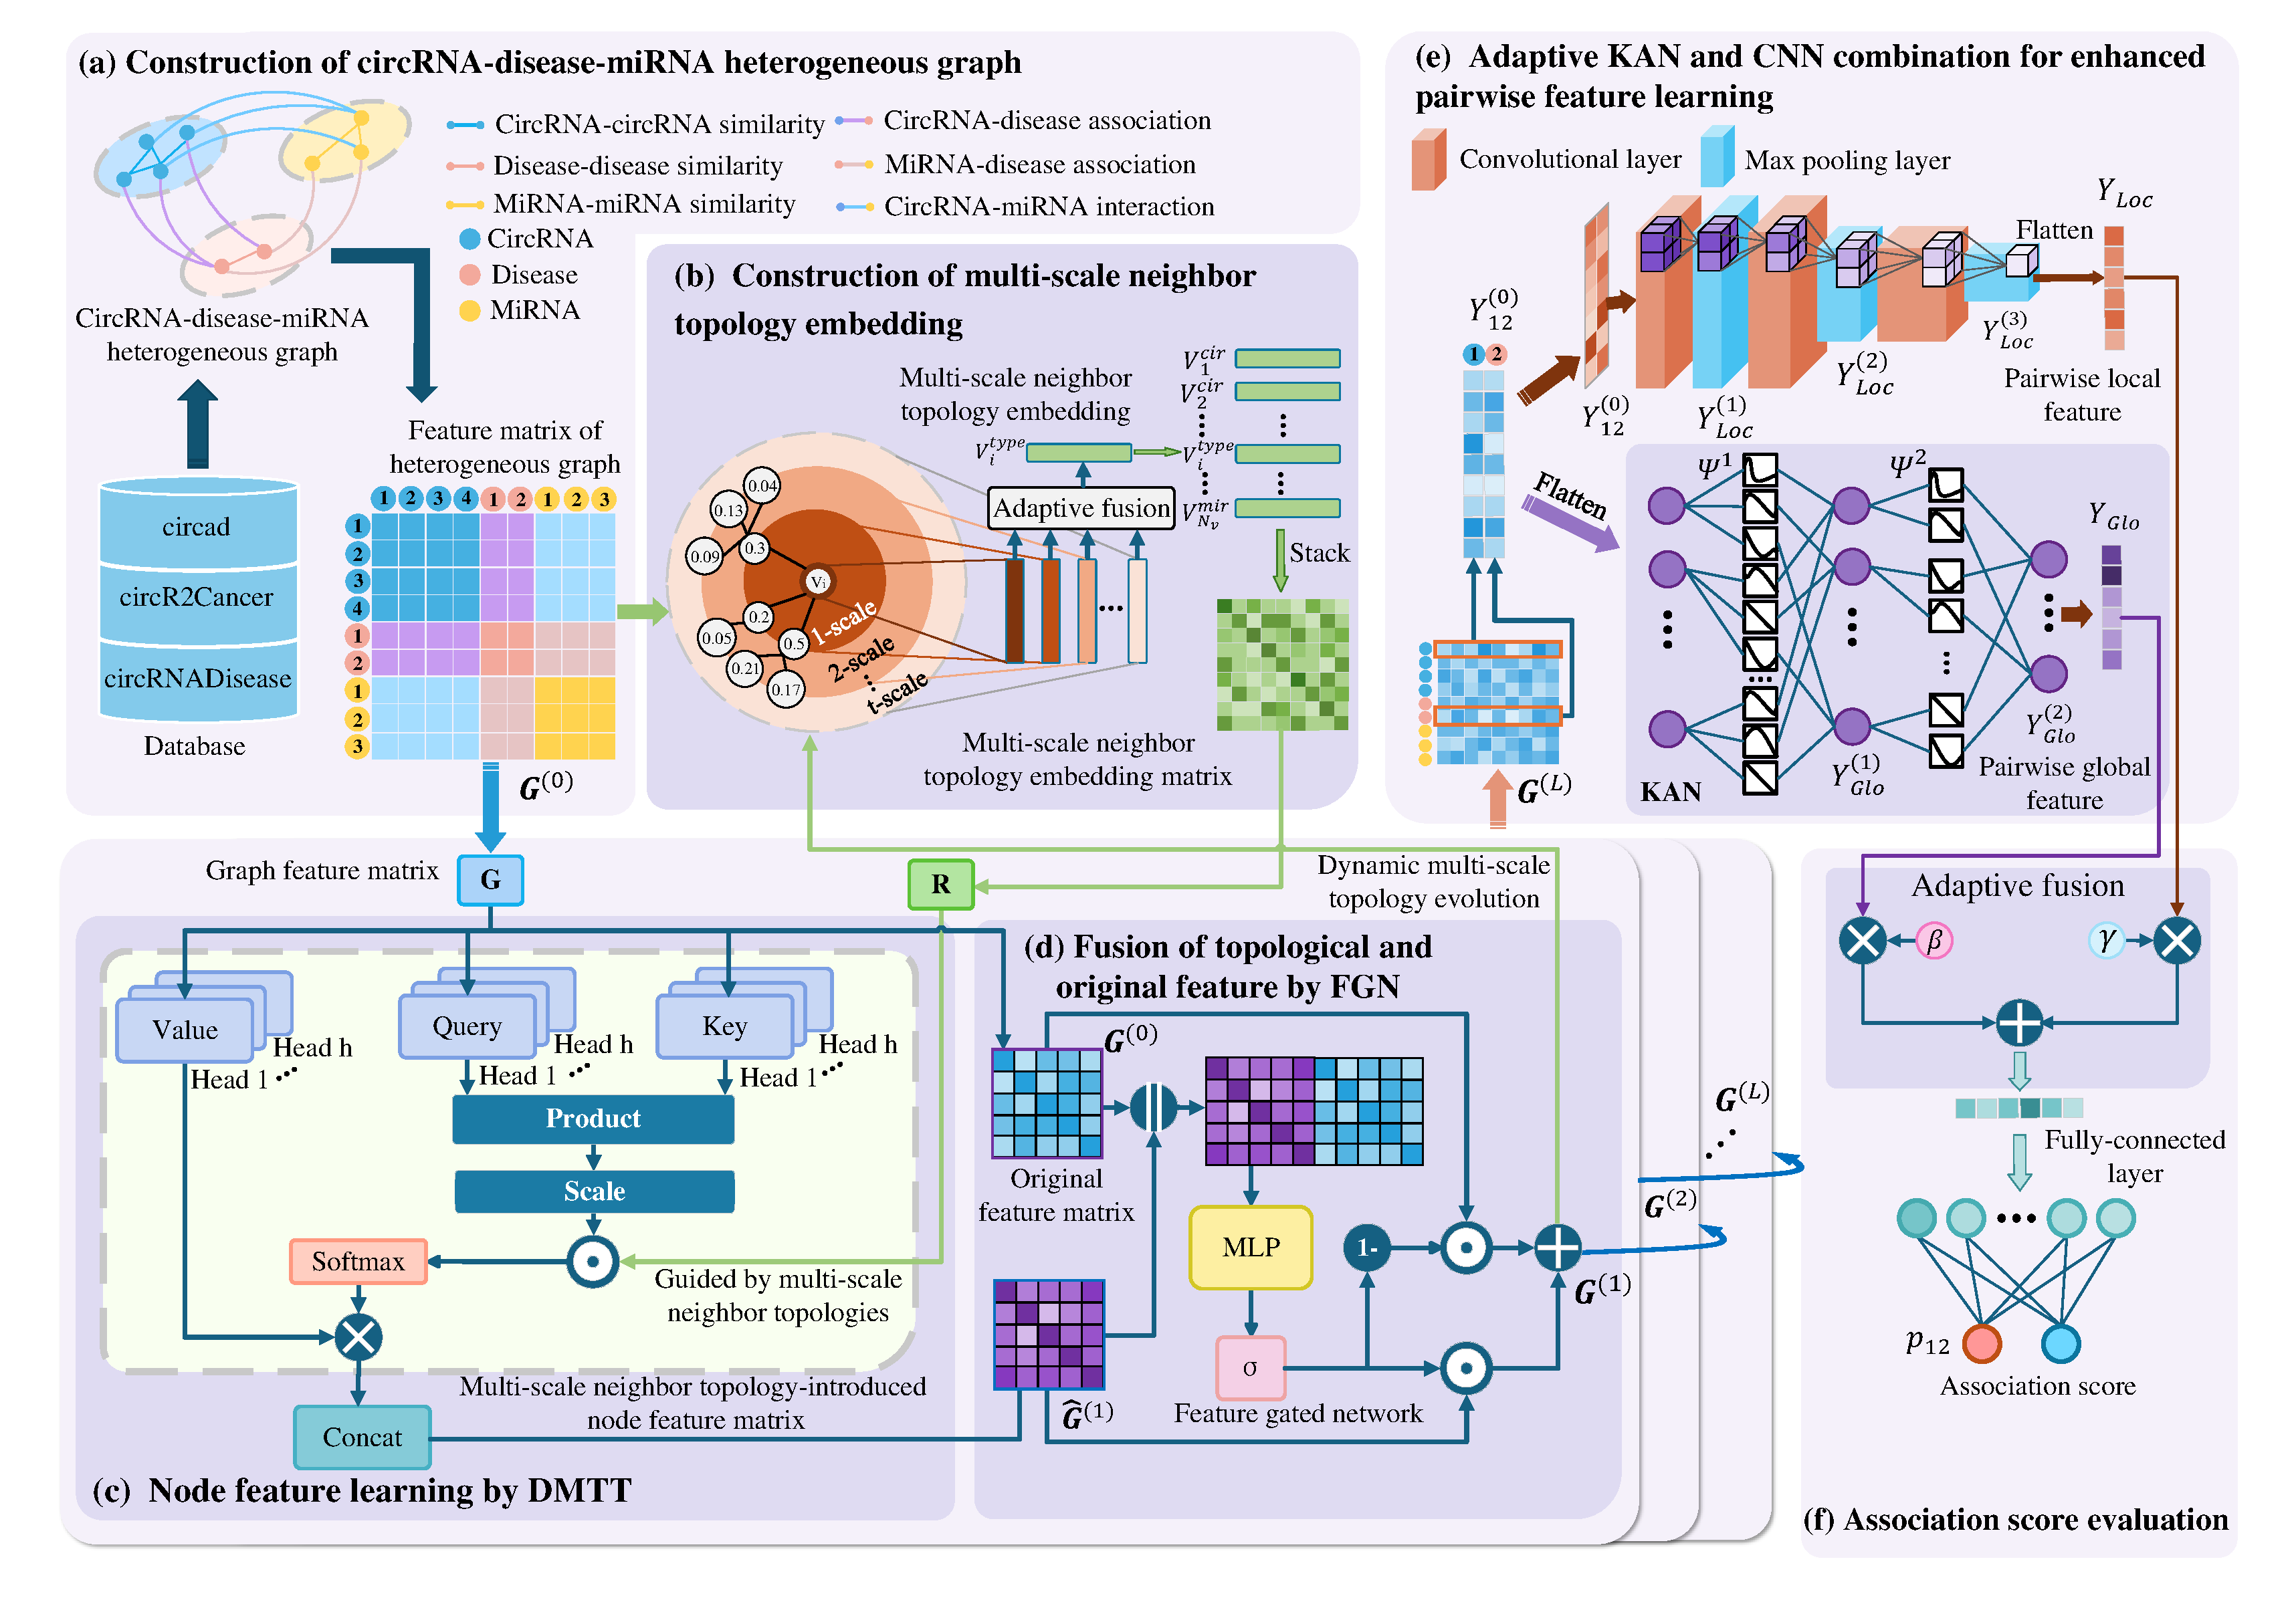
\includegraphics[width=6.9in]{fig/visio1.pdf}\\
	\caption{The overall framework of MKCD. {\textbf{(a)} Construction of the circRNA-disease-miRNA heterogeneous graph. \textbf{(b)} Adaptive multi-scale neighbor topology embedding construction strategy. \textbf{(c)} Learn the complex relationships among circRNA, miRNA, and disease nodes based on DMTT. \textbf{(d)} Fuse topological features and original node features by FGN. \textbf{(e)} Learn local and global dependencies of features of circRNA and disease node pairs based on ACK. \textbf{(f)} Adaptively fuse two representations and estimate circRNA-disease association scores.}}
    \label{fig:visio1}
	\vspace{-0.4cm}
\end{figure*}

\section{Materials and methods}
We propose a novel prediction model, MKCD (Figure \ref{fig:visio1}), for predicting disease-related circRNA candidates. A circRNA-disease-miRNA heterogeneous graph is constructed to integrate the similarities, interactions, and associations among circRNA, disease, and miRNA (Figure \ref{fig:visio1}(a)). MKCD consists of four components, each learning distinct information from the heterogeneous graph. The proposed DMTT encodes the complex relationships among multiple circRNA, disease, and miRNA nodes (Figure \ref{fig:visio1}(c)). It further guides the transformer model's learning process through dynamically constructed multi-scale neighbor topology embeddings via AMNE (Figure \ref{fig:visio1}(b)). To preserve more detailed information from node features, we introduce FGN (Figure \ref{fig:visio1}(d)). The designed ACK is used to learn and fuse both global and local dependencies between the features of circRNA and disease node pairs (Figure \ref{fig:visio1}(e)). These components work together to improve the capability of MKCD in predicting circRNA-disease associations.

\subsection{Dataset}

The dataset utilized in this study is derived from previous work \cite{lan2022kgancda}, which comprises two datasets containing circRNA, disease and miRNA information. The first dataset covers 514 circRNAs, 62 diseases, and 564 miRNAs. The second dataset contains associations and interactions among 330 circRNAs, 79 diseases, and 245 miRNAs. We integrated these two datasets to form a new, larger dataset. This merged dataset consists of 989 circRNA-disease associations, 837 miRNA-disease associations, and 902 circRNA-miRNA interactions, covering a total of 834 circRNAs, 138 diseases, and 555 miRNAs. The original associations between circRNAs and diseases are obtained from the circR2Cancer database \cite{lan2020circr2cancer}, the circad database \cite{rophina2020circad}, and the circRNADisease database \cite{zhao2018circrna}.

\subsection{CircRNA-disease-miRNA heterogeneous graph}

\begin{figure*}[!t]
	\centering
	%\usepackage{float}
	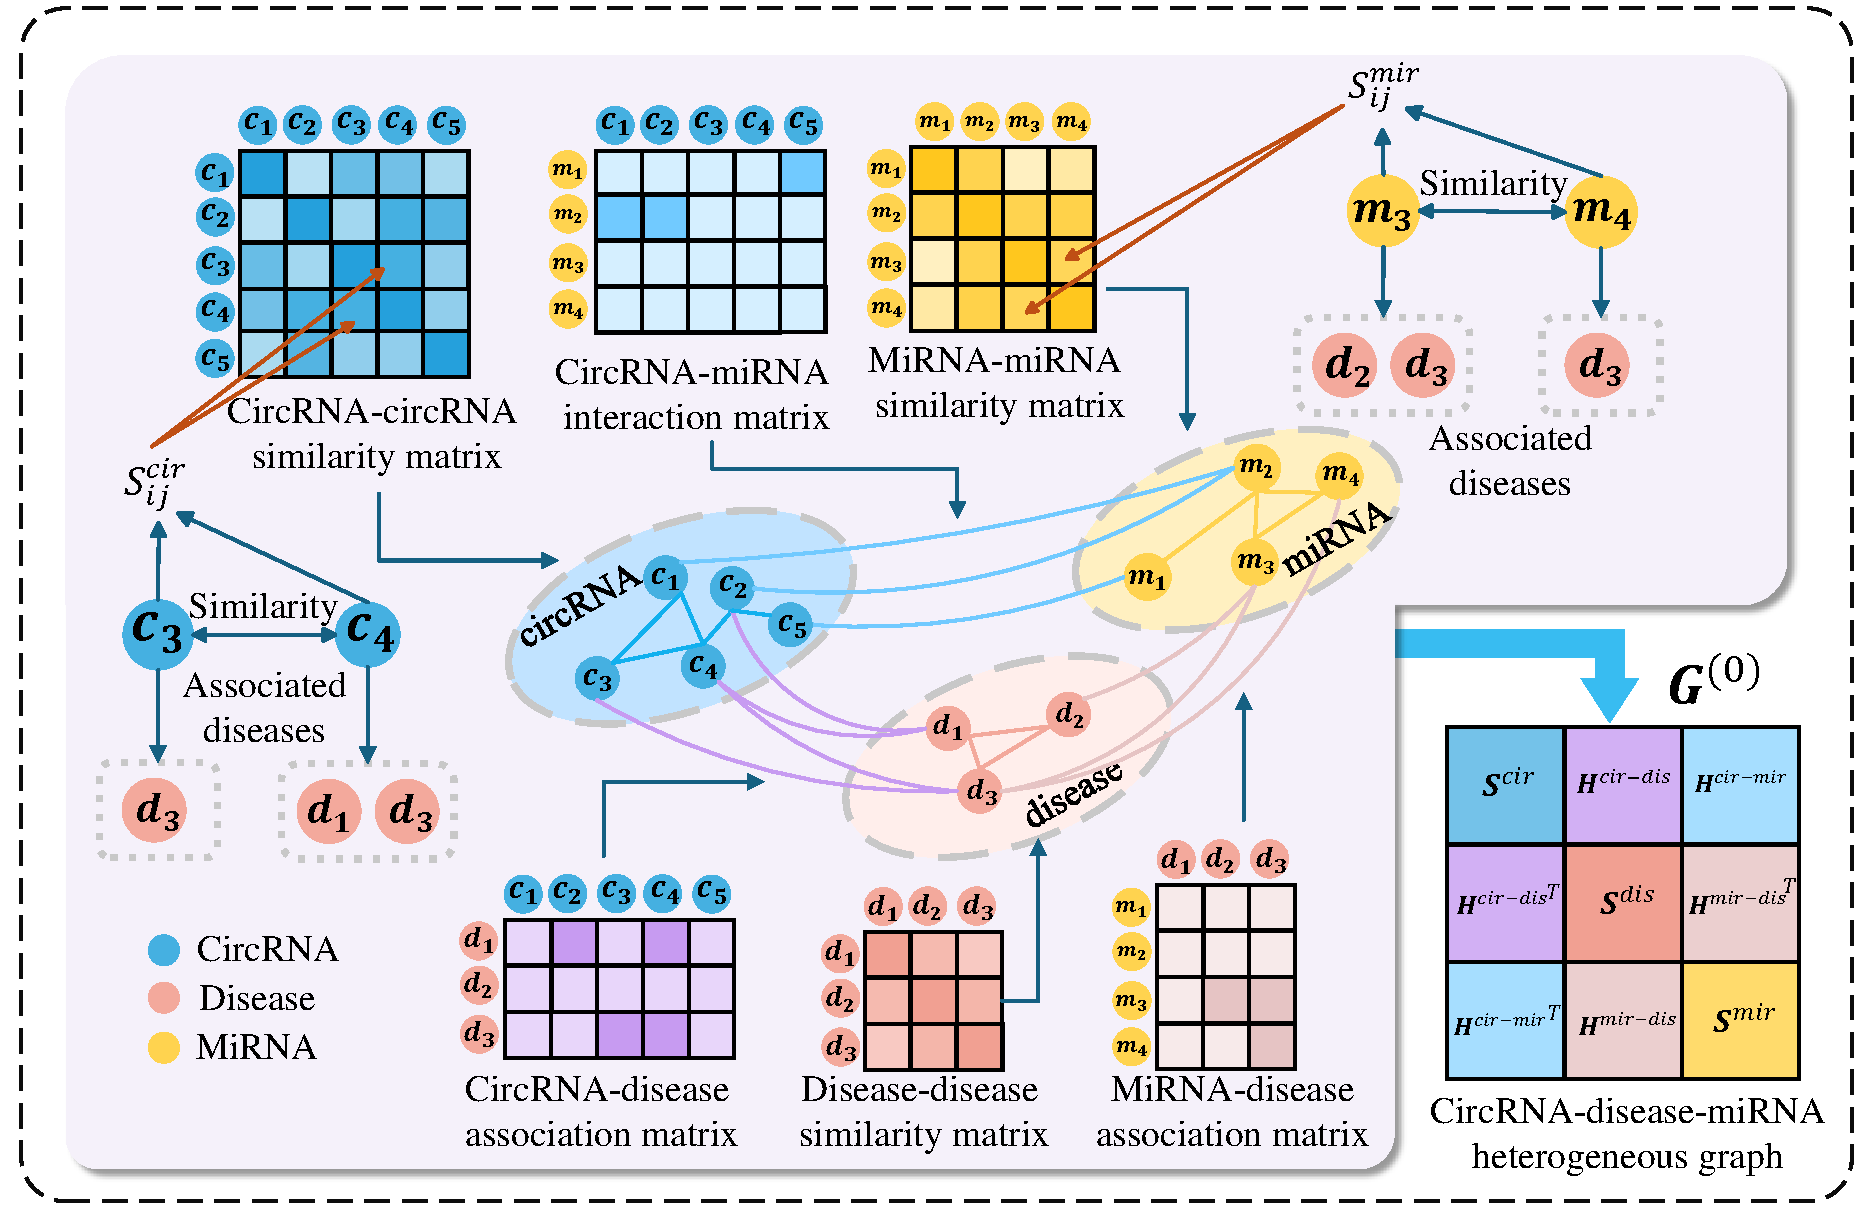
\includegraphics[width=5in]{fig/visio2.pdf}\\
	\caption{Construction of the circRNA-disease-miRNA heterogeneous graph based on multi-source data.}
	\label{fig:visio2}
	\vspace{-0.4cm}
\end{figure*}

We constructed a three-layer heterogeneous graph $\mathcal{G}=(\mathcal{V}, \mathcal{E})$ using associations, interactions, and similarities among circRNAs, miRNAs, and diseases (Figure \ref{fig:visio2}). The node set $\mathcal{V}=\{V^{cir}\cup V^{dis}\cup V^{mir}\}$ comprises the set of circRNA nodes $V^{cir}$, disease nodes set $V^{dis}$, and miRNA nodes set $V^{mir}$. An edge $e_{ij} \in \mathcal{E}$ connects a pair of nodes $v_i,v_j \in \mathcal{V}$, represented by the association and interaction matrix $H$ and similarity matrix $S$.

The association and interaction matrix $H$ among circRNAs, miRNAs, and diseases is defined as follows,
\begin{equation}
H = \left\{ \begin{array}{l}
{H^{cir-dis}} \in {\mathbb{R}^{N_{cir}\times N_{dis}}}, \text{ if } {v_i} \in {V^{cir}}, {v_j} \in {V^{dis}};\\[5pt]
{H^{mir-dis}} \in {\mathbb{R}^{N_{mir}\times N_{dis}}}, \text{ if } {v_i} \in {V^{mir}}, {v_j} \in {V^{dis}};\\[5pt]
{H^{cir-mir}} \in {\mathbb{R}^{N_{cir}\times N_{mir}}}, \text{ if } {v_i} \in {V^{cir}}, {v_j} \in {V^{mir}};\\
\end{array} \right.
\end{equation}
where $H^{cir-dis}$, $H^{mir-dis}$, and $H^{cir-mir}$ denote the circRNA-disease association matrix, miRNA-disease association matrix, and circRNA-miRNA interaction matrix, respectively. $N_{cir}$, $N_{dis}$, and $N_{mir}$ represent the number of circRNAs, diseases, and miRNAs in the dataset. 
$H_{ij} \in H^{cir-dis} (H^{mir-dis})$ represents the association between the circRNA (miRNA) node $v_i^{cir}(v_i^{mir})$ and the disease node $v_j^{dis}$. For a circRNA (miRNA) node $v_i^{cir}$ ($v_i^{mir}$) and a disease node $d_j^{dis}$, if $H_{ij}^{cir-dis}=1$ ($H_{ij}^{mir-dis}=1$), it indicates the existence of an association between them; conversely, $H_{ij}^{cir-dis}=0$ ($H_{ij}^{mir-dis}=0$), no association has been observed. If $H_{ij}^{cir-mir}=1$, an interaction is present between the circRNA node $v_i^{cir}$ and the miRNA node $v_j^{mir}$; otherwise, $H_{ij}^{cir-mir}=0$.


$S$ represents the similarity matrix related to circRNAs, miRNAs, and diseases,
\begin{equation}
S = \left\{ \begin{array}{l}
{S^{cir}} \in {\mathbb{R}^{N_{cir}\times N_{cir}}}, \text{ if } {v_i},{v_j} \in {V^{cir}};\\[5pt]
{S^{dis}} \in {\mathbb{R}^{N_{dis}\times N_{dis}}}, \text{ if } {v_i},{v_j} \in {V^{dis}};\\[5pt]
{S^{mir}} \in {\mathbb{R}^{N_{mir}\times N_{mir}}}, \text{ if } {v_i},{v_j} \in {V^{mir}};\\
\end{array} \right.
\end{equation}
where $S^{cir}$, $S^{dis}$, and $S^{mir}$ are the similarity matrix for circRNAs, diseases, and miRNAs, respectively. The values in $S^{cir}$, $S^{dis}$, and $S^{mir}$ range from 0 to 1, reflecting similarity between two nodes of the same type, with higher values indicating greater similarity.

According to the method proposed by Wang {\it et al.} \cite{wang2010inferring}, the similarity between two disease nodes $[v_i^{dis},v_j^{dis}]$ is calculated based on their directed acyclic graph (DAG). The similarities of circRNAs and miRNAs are calculated using the methods proposed by Wang {\it et al.} \cite{wang2010inferring} and Chen {\it et al.} \cite{chen2015constructing}, respectively, where the similarity of a pair of circRNAs (miRNAs) is derived from the similarity between the two sets of diseases associated with them. For instance, suppose the $i$-th circRNA node $v_i^{cir}$ is associated with $N^{cir}_i$ diseases, which forms the set $\Omega_i^{cir} = \{d_{ik} | k = 1, \ldots, N^{cir}_i\}$, and the $j$-th circRNA node $v_j^{cir}$ is associated with the disease set $\Omega_j^{cir} = \{d_{jl} | l = 1, \ldots, N^{cir}_j\}$. The similarity $S_{ij}^{cir}$ between $[v_i^{cir},v_j^{cir}]$ is determined by evaluating the similarity between $\Omega_i^{cir}$ and $\Omega_j^{cir}$, 
\begin{equation}
S_{ij}^{cir} = \frac{{\sum_{m=1}^{N^{cir}_i}S_m}+{\sum_{n=1}^{N^{cir}_j}}S_n }{N^{cir}_j + N^{cir}_j},
\end{equation}
\begin{equation}
    S_m = \underset{1\leqslant n\leqslant N^{cir}_j}{\max}(DS(d_{im}, d_{jn})),
\end{equation}
\begin{equation}
    S_n = \underset{1\leqslant m\leqslant N^{cir}_i}{\max}(DS(d_{jn}, d_{im})),
\end{equation}
where $DS(d_{im}, d_{jn})$ is the semantic similarity between diseases $d_{im}$ and $d_{jn}$ which belong to $\Omega_i^{cir}$ and $\Omega_j^{cir}$ respectively. %* 
Similarly, we can calculate the similarity $S_{ij}^{mir}$ for $[v_i^{mir},v_j^{mir}]$.

Based on the constructed association (interaction) matrix $H$ and the similarity matrix $S$, the original feature matrix of the heterogeneous graph $G^{(0)} \in \mathbb{R}^{N_v\times N_v}$ is defined as follows,
\begin{equation}
G^{(0)} = \left[\ \begin{array}{lll}
S^{cir} & H^{cir-dis} & H^{cir-mir}\\
{H^{cir-dis}}^T & S^{dis} & {H^{mir-dis}}^T\\
{H^{cir-mir}}^T & H^{mir-dis} & S^{mir}\\
\end{array} \right],
\end{equation}
where $N_v$ denotes the total number of circRNAs, miRNAs, and diseases, and ${H^{cir-dis}}^T$ represents the transpose of the matrix $H^{cir-dis}$. The $i$-th row $g_i$ of the matrix $G^{(0)}$ represents the node embedding of node $v_i \in \mathcal{V}$, which contains the associations and similarities involving $v_i$ and all circRNAs, diseases, and miRNAs. The set $\{g_i | 0 \leqslant i < N_{cir}\}$ denotes the collection of node embeddings for all circRNAs. Furthermore, the sets $\{g_i | N_{cir} \leqslant i < N_{cir} + N_{dis}\}$ and $\{g_i | N_{cir} + N_{dis} \leqslant i < N_{cir} + N_{dis} + N_{mir}\}$ represent the collections of node embeddings for all diseases and miRNAs, respectively.


\subsection{Adaptive multi-scale neighbor topology embedding construction strategy (AMNE)}

\begin{figure}
    \centering
    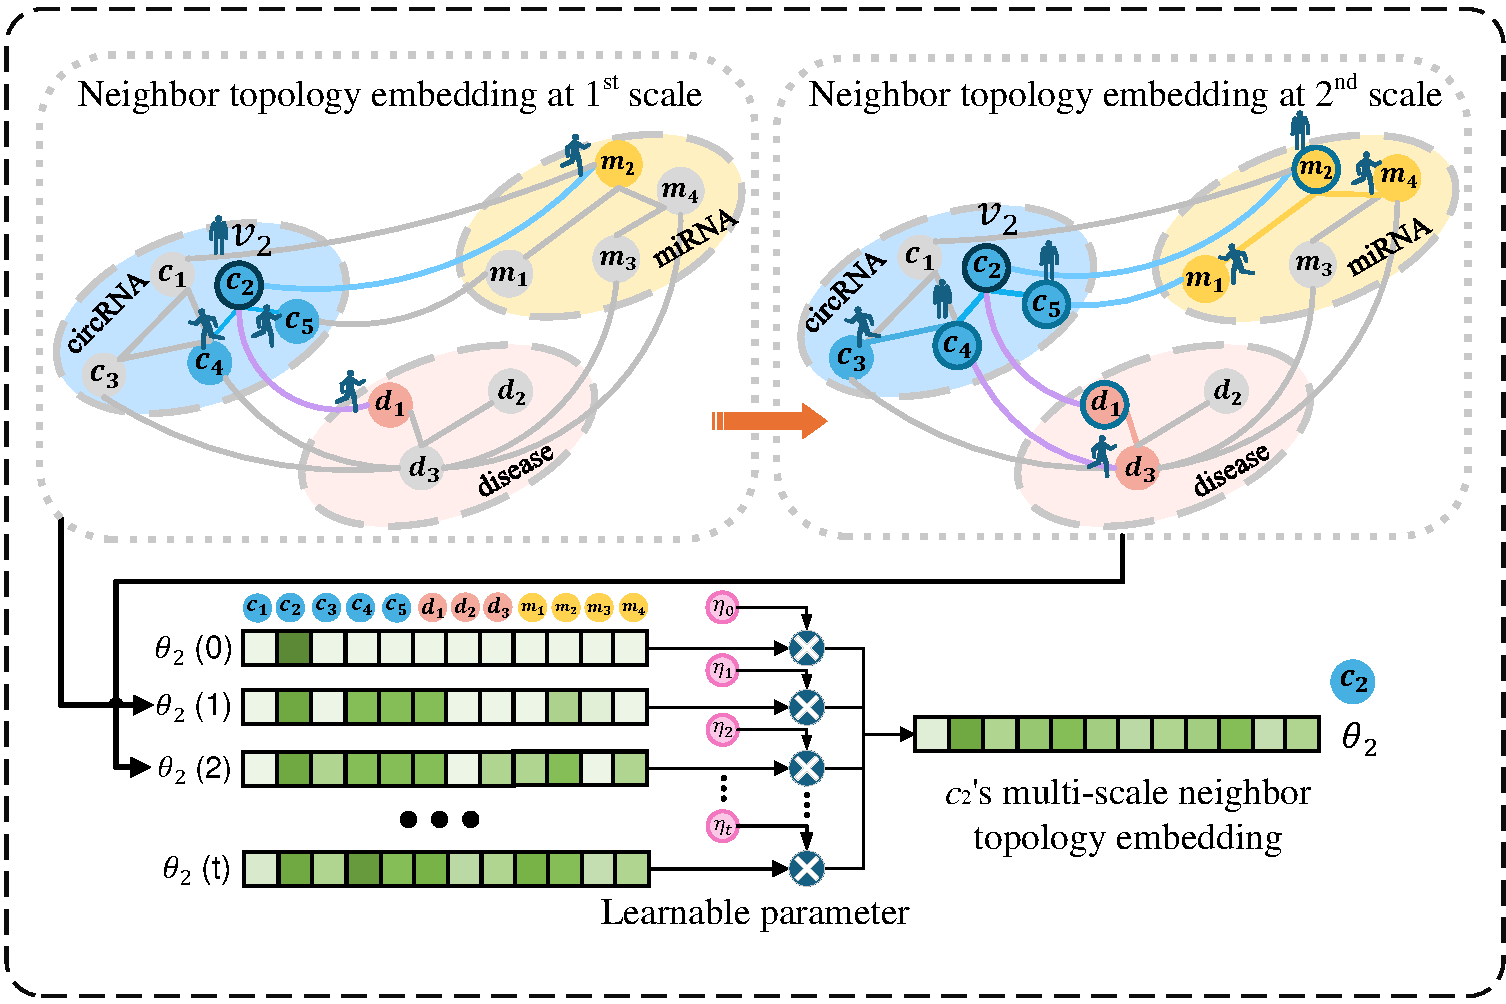
\includegraphics[width=3.5in]{fig/visio3.pdf}\\       
	\caption{Process of adaptively constructing multi-scale neighbor topology embeddings with RWR, illustrated by node $c_{2}$.}
    \label{fig:visio3}
	\vspace{-0.4cm}
\end{figure}


In the circRNA-disease-miRNA heterogeneous graph, the node $v_i$ has one-scale neighbors that can be reached in one step, or $d$-scale neighbors that can be reached in $d\ (d > 1)$ steps. The multi-scale neighbor topological structure formed by these neighboring nodes can provide important auxiliary information for predicting the associations between circRNAs and diseases. The contributions of low-scale (one-scale) neighbors and high-scale ($d$-scale) neighbors to the features learned for each node are different, thus, we proposed AMNE, which utilizes random walk with restart (RWR) to establish multi-scale neighbor topology embeddings (Figure \ref{fig:visio3}). Taking $v_i$ as an example, the walker starts from $v_i$ and performs random walks to travel to other nodes in the circRNA-disease-miRNA heterogeneous graph. The probability distribution of reaching all circRNA, disease, and miRNA nodes at time $t$ is given by $\theta _i{(t)} \in \mathbb{R}^{1 \times N_v}$,
\begin{equation}
\theta _i{(t)} = (1 - \lambda) O^T \theta _i{(t-1)} + \lambda \theta _i{(0)},
\label{eq:eq4}
\end{equation}
where the $j$-th value of $\theta _i{(t)}$ denotes the probability that the walker starts from $v_i$ reaches node $v_j$ $(0 \leqslant j < N_v)$ after $t$ steps. $\theta _i{(0)}$ is the initial one-hot vector, where the $i$-th position is 1 and all other positions are 0. $\lambda$ is the probability that the walker restarts from the starting point; a larger value of $\lambda$ results in a smaller movement range of the walker within the network. $O \in \mathbb{R}^{N_v \times N_v}$ is obtained from the row-normalized matrix of $G^{(0)}$, where $o_{ij} \in O$ represents the transition probability from $v_i$ to $v_j$. $\theta _i{(t)}$ can be viewed as the probability distribution of reaching various nodes after $t$ steps from $v_i$, thus it serves as the $t$-scale neighbor topology embedding of $v_i$.

According to Eq. (\ref{eq:eq4}), we can build neighbor topology embeddings from scale 0 to scale $r$. These scale neighbor topology embeddings are adaptively fused to obtain the multi-scale neighbor topology embedding $\theta _i$ for $v_i$,
\begin{equation}
\label{eq:eq5}
\theta _i = \eta_0  \theta _i{(0)} + \eta_1 \theta _i{(1)} + \cdots + \eta_k \theta _i{(k)} + \cdots + \eta_t \theta _i{(r)},
\end{equation}
where $\eta_k \in (0, 1)$ are randomly initialized learnable parameters, and $\sum_{k=0}^{t}\eta_k = 1$.

After applying AMNE for each $v_i(0 \leqslant i < N_v)$, we can obtain the multi-scale neighbor embedding for all nodes. These embeddings are stacked vertically to form the embedding matrix $R \in \mathbb{R}^{N_v \times N_v}$,
\begin{equation}
\label{eq:eq6}
	R = \left[\begin{array}{cccc}
		\theta _0\\
		\theta _1\\
		\vdots\\
		\theta _{N_v-1}
	\end{array}\right].
\end{equation}

%2.4
\subsection{Node feature learning based on DMTT}

Typically, multiple circRNAs and miRNAs form interactions and collaboratively participate in the processes of various diseases. Therefore, there are close relationships among the features of multiple circRNAs, miRNAs, and disease nodes, making it necessary to establish a self-attention mechanism to capture these relationships. Traditional transformers focus solely on the similarities between node features and do not fully exploit the topological structures formed between nodes, especially the multi-scale neighbor topological structures. Inspired by the transformer proposed by Vaswani {\it et al.} \cite{vaswani2017attention}, we introduce a DMTT (dynamic multi-scale neighbor topology-guided transformer) mechanism (Figure \ref{fig:visio4}) that utilizes the multi-scale neighbor topology embeddings established by AMNE to guide the learning of attention scores.

We use a multi-head attention mechanism to prevent single-head attention from getting stuck in local optima during training, reducing bias in the learning process. %*
For the $m$-th attention head, we first establish the query matrix $Q_{m}^{(l)} \in \mathbb{R}^{N_v \times \frac{N_v}{h}}$, the key matrix $K_{m}^{(l)} \in \mathbb{R}^{N_v \times \frac{N_v}{h}}$, and the value matrix $V_{m}^{(l)} \in \mathbb{R}^{N_v \times \frac{N_v}{h}}$ as follows,
\begin{equation}
	\begin{aligned}
		{Q_{m}^{(l)}} &= G^{{(l - 1)}}{W_{m}^{Q{(l)}}} \\
		{K_{m}^{(l)}} &= G^{{(l - 1)}}{W_{m}^{K{(l)}}} ,\\
		{V_{m}^{(l)}} &= G^{(l - 1)}{W_{m}^{V{(l)}}}
	\end{aligned}
\end{equation}
where $G^{(l - 1)} \in \mathbb{R}^{N_v \times N_v}$ is the feature matrix of the graph nodes that are input at layer $l$ $(1 \leqslant l \leqslant L)$. When $l = 1$, $G^{(0)}$ represents the original feature matrix, and $h$ is the number of attention heads. $Q_{m}^{(l)}$, $K_{m}^{(l)}$, and $V_{m}^{(l)}$ are obtained from $G^{(l - 1)}$ through different linear projections, with $W_{m}^{Q{(l)}}$, $W_{m}^{K{(l)}}$, and $W_{m}^{V(l)} \in \mathbb{R}^{N_v \times \frac{N_v}{h}}$ being the corresponding weight matrices for the linear projections. Then, we perform a dot product operation on $Q_{m}^{(l)}$ and ${K_{m}^{(l)}}^T$ to obtain the attention score matrix ${S_{m}^{(l)}} \in \mathbb{R}^{N_v \times N_v}$,
\begin{equation}
	{S_{m}^{(l)}} = \frac{Q_{m}^{(l)}{K_{m}^{(l)}}^T}{\sqrt{d}},
\end{equation}
where $d = \frac{N_v}{h}$ and $\sqrt{d}$ is a scaling factor used to adjust the magnitude of the attention scores to enhance numerical stability during the training process. The $i$-th row of $S_{m}^{(l)}$ records the attention scores from all circRNA, disease, and miRNA nodes to $v_i$.

After the $(l-1)$th layer of DMTT encoding, the topology between the nodes has changed. According to Eq. \ref{eq:eq4}, we perform row normalization on $G^{(l - 1)}$ to obtain the new $O^{(l)}$. A random walk is then conducted from each node as the starting point, i.e., Eq. \ref{eq:eq4} is executed again, resulting in new neighbor topology embeddings at different scales, which are adaptively fused into a new multi-scale neighbor topology embedding $\theta_i^{(l)}$ (Eq. \ref{eq:eq5}). $\theta_i^{(l)}$ is vertically stacked to obtain the embedding matrix $R^{(l)}$ of the dynamically evolved layer (Eq. \ref{eq:eq6}). %*
The $i$-th row of $R^{(l)}$ records the neighbor topology of $v_i$ with all other circRNA, disease, and miRNA nodes after the $(l-1)$th layer transformer encoding. We perform a Hadamard product operation between $R^{(l)}$ and $S_{m}^{(l)}$. This approach allows the multi-scale neighbor topology embeddings to guide the learning of attention scores. We establish the multi-scale neighbor topology-introduced attention score matrix $\widetilde{S}_{m}^{(l)} \in \mathbb{R}^{N_v \times N_v}$ as follows,
\begin{equation}
	\widetilde{S}_{m}^{(l)} = S_{m}^{(l)} \odot R^{(l)},
\end{equation}
where $\odot$ denotes the Hadamard product operation. Multiplying $\widetilde{S}_{m}^{(l)}$ with $V_{m}^{(l)}$ produces the node features ${Z_{m}^{(l)}} \in \mathbb{R}^{N_v \times \frac{N_v}{h}}$ learned by the $m$-th attention head,
\begin{equation}
	{Z_{m}^{(l)}} = softmax(\widetilde{S}_{m}^{(l)})V_{m}^{(l)}.
\end{equation}
Finally, by concatenating the node features learned by all $h$ attention heads, we obtain the multi-scale neighbor topology-introduced node feature matrix $\hat{G}^{(l)} \in \mathbb{R}^{N_v \times N_v}$ for layer $l$,
\begin{equation}
	\hat{G}^{(l)}= \bigg\|_{\substack{m\in {[1,h]}}} Z^{(l)}_{m},
\end{equation}
where $\|$ denotes the concatenation operation. The $i$-th row of $\hat{G}^{(l)}$ records the features of $v_i$ learned at layer $l$.
%2.5

\subsection{Fusion of multiple types of features based on FGN}
In DMTT, the feature matrix ${G}^{(l - 1)}$ that is input at layer $l$ contains more detailed information about each node, while the feature matrix $\hat{G}^{(l)}$ learned based on DMTT places greater emphasis on the information guided by multi-scale neighbor topology embedding. Therefore, it is necessary to incorporate ${G}^{(l - 1)}$ into the feature learning process at layer $l$. To integrate the information contained in $\hat{G}^{(l)}$ and $G^{(l - 1)}$, we establish an FGN (feature-gated network) after DMTT at layer $l$, with the weight matrix denoted as $\alpha^{(l)}$,
\begin{equation}
    \alpha^{(l)} = \sigma (W^{gate(l)}(\hat{G}^{(l)}\| G^{(l - 1)}) + b^{gate(l)}),
\end{equation}
where $W^{gate(l)}$ and $b^{gate(l)}$ are learnable weight matrices and bias, and $\sigma$ is the Sigmoid activation function. All parameters of the FGN are randomly initialized and are learnable during the training process, allowing it to discern the more significant features in $\hat{G}^{(l)}$ and $G^{(l - 1)}$.

The FGN-enhanced node feature representation is denoted as ${G}^{(l)} \in \mathbb{R}^{N_v \times N_v}$,
\begin{equation}
    {G}^{(l)} =  \alpha^{(l)} \odot \hat{G}^{(l)} + (1 - \alpha^{(l)}) \odot G^{(l - 1)},
\end{equation}
where $\odot$ denotes the Hadamard product operation. When $l \neq L$, $G^{(l)}$ will serve as the input for the next layer of DMTT, where $l = L$, $G^{(L)}$ represents the final node feature representation matrix.



%2.6
\subsection{Adaptive joint CNNs and KAN enhanced pairwise feature learning strategy}

\begin{figure}
    \centering
    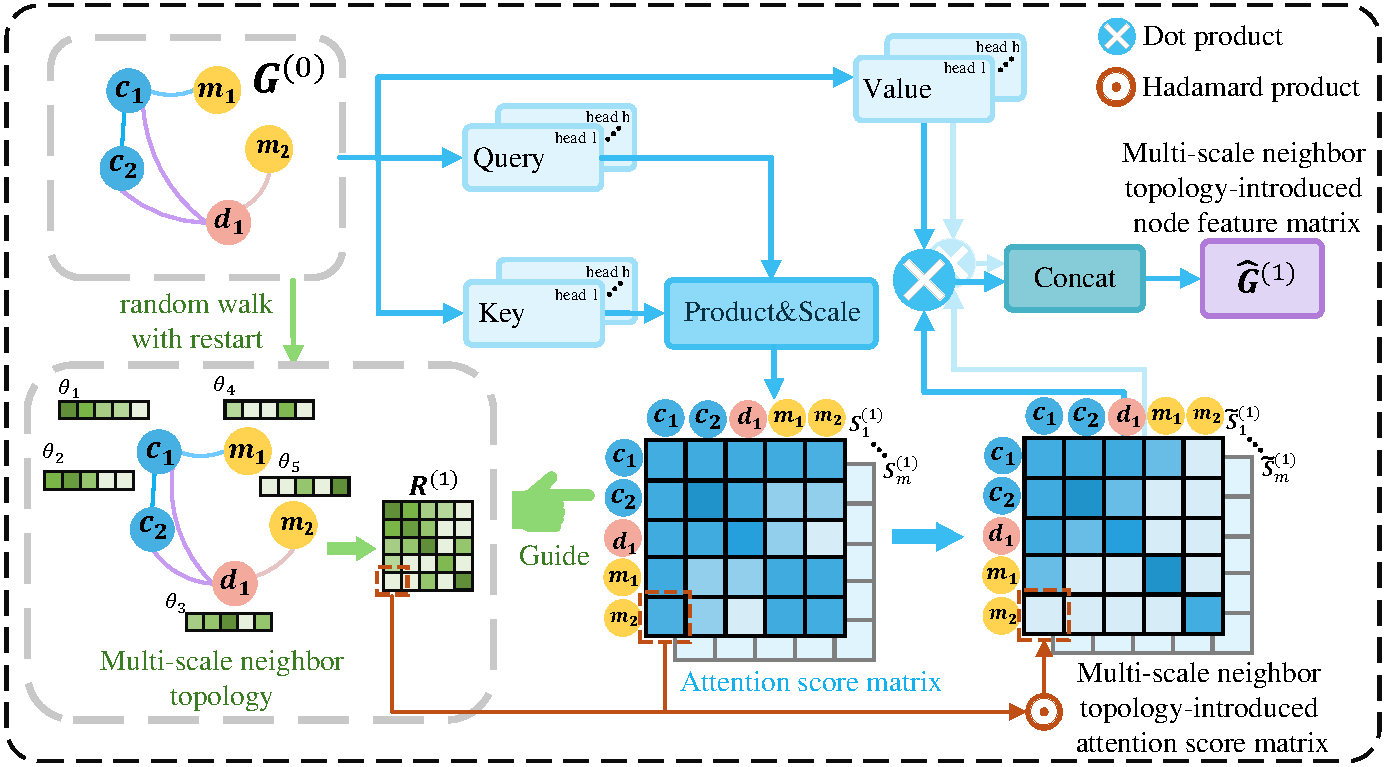
\includegraphics[width=3.5in]{fig/visio4.pdf}\\       
	\caption{Illustration of node feature learning process guided by multi-scale neighbor topology, using $G^{(0)}$ as an example.}
    \label{fig:visio4}
	\vspace{-0.4cm}
\end{figure}

If the circRNA node $v_i^{cir}$ and the disease node $d_j^{dis}$ have similarities, associations, or interactions with the same circRNAs, diseases, and miRNAs, then the node pair $[v_i^{cir}, d_j^{dis}]$ is more likely to be associated. Based on this biological premise, we vertically stack the feature representations obtained from the FGN-enhanced DMTT for both circRNA and disease nodes, forming a node pair-level feature representation ${Y_{ij}^{(0)}} \in \mathbb{R}^{2 \times N_v}$,
\begin{equation}
    {Y_{ij}^{(0)}} = \begin{bmatrix} {G^{(L)}_i} \\ {G^{(L)}_j} \end{bmatrix},
\end{equation}
where the sets $\{G^{(L)}_{i} | 0 \leqslant i < N_{cir}\}$ and $\{G^{(L)}_j | N_{cir} \leqslant j < N_{cir} + N_{dis}\}$ represent the node feature representations of all circRNAs and diseases in $G^{(L)}$, respectively.

The ACK (adaptive joint CNNs and KAN learning strategy) we designed will further extract the information within the circRNA-disease node pairs. The KAN module we established learns the pairwise node representations from a global perspective, while the CNN module focuses more on extracting local information of the pairwise node representations.

\subsubsection{Pairwise global feature learning based on KAN}
Compared to the multi-layer perceptron (MLP), KAN replaces weight parameters and activation functions with learnable functions to adaptively learn the weights of the connections between neurons. This learnable function is typically composed of multiple stacked spline functions, enabling the KAN network to better capture the complex relationships among the features in ${Y_{ij}^{(0)}}$. Through multiple layers of the KAN network, a feature representation of the node pair $[v_i^{cir}, d_j^{dis}]$ is learned from a global perspective. The input feature representation of the node pair at the $l$-th layer $Y_{Glo}^{(l - 1)}$ is transformed into the pairwise global feature representation ${Y}_{Glo}^{(l)}$ after passing through the $l$-th layer of the global feature learning module based on the KAN network,
\begin{equation}
    {Y}_{Glo}^{(l)} = KAN^{(l)}(Y_{Glo}^{(l - 1)}) = \varPsi^{(l)}(Y_{Glo}^{(l - 1)}),
\end{equation}
where $KAN^{(l)}$ denotes the $l$-th KAN layer. When $l=1$, $Y_{Glo}^{(0)}$ is obtain by flattening the original circRNA-disease node pair-level feature representation $Y_{ij}^{(0)}$. When $l=L$, $Y_{Glo}^{(L)}$ represents the final pairwise global feature representation ${Y}_{Glo} \in \mathbb{R}^{1\times f}$, where $f$ is the feature dimension. 

The matrix $\varPsi^{(l)}$ is composed of learnable functions for the $l$-th KAN layer, containing a total of $n^{(l - 1)} \times n^{(l)}$ learnable functions. Therefore, $\varPsi^{(l)}$ is defined as,
\begin{equation}
    \varPsi^{(l)} = \left(
    \begin{array}{cccc}
        \psi_{1,1} & \psi_{1,2} & \cdots & \psi_{1,n^{(l-1)}} \\
        \psi_{2,1} & \psi_{2,2} & \cdots & \psi_{2,n^{(l-1)}} \\
        \vdots & \vdots & \ddots & \vdots \\
        \psi_{n^{(l)},1} & \psi_{n^{(l)},2} & \cdots & \psi_{n^{(l)},n^{(l-1)}}
    \end{array}
    \right),
\end{equation}
where $n^{(l - 1)}$ and $n^{(l)}$ represent the number of neurons in the $(l - 1)$th and $l$-th layers, respectively. The $\psi_{i,j}$ represents the learnable function associated with the edge connecting the $j$-th neuron $z^{(l-1)}_j (1\leqslant j\leqslant n^{(l-1)})$ in the $(l-1)$th layer to the $i$-th neuron $z^{(l)}_i (1\leqslant i\leqslant n^{(l)})$ in the $l$-th layer. The output neuron $z^{(l)}_i$of the $l$-th layer is,
\begin{equation}
    z^{(l)}_i = \sum_{j = 1}^{n^{(l-1)}}  \psi_{i,j}(z^{(l-1)}_j),
\end{equation}
where the $\psi_{i,j}$ is composed of a basis function and a B-spline function,
\begin{equation}
    \psi_{i,j}(z^{(l-1)}_j) = \omega^{b}_{i,j}b(z^{(l-1)}_j) + \omega^{s}_{i,j}spline_{i,j}(z^{(l-1)}_j),
\end{equation}
\begin{equation}
    spline_{i,j} = \sum_{k = 1}^{n_{grid}}c_{k} B_{k},
\end{equation}
where $b$ is the basis function ${SiLU}$, and $\omega^{b}_{i,j}$ and $\omega^{s}_{i,j}$ are learnable weight parameters. The B-spline function $spline_{i,j}$ is a linear combination of $n_{grid}$ B-spline basis functions $B_{k}$, with learnable coefficients $c_{k}$.

\subsubsection{Pairwise local feature learning based on CNNs}

We have established CNNs to learn the local features of circRNA-disease node pairs. In the CNNs, each block consists of a convolution layer followed by a pooling layer. In the $l$-th block $(1 \leqslant d \leqslant D)$, given the feature representation of a circRNA-disease node pair ${Y}_{Loc}^{(d - 1)}$, we use the convolution and pooling operations to extract its pairwise local features ${Y}_{Loc}^{(d)}$,
\begin{equation}
{Y}_{Loc}^{(d)} = max(\mathop{\rm{\tau}}({W_{conv}^{(d)}}  * {Y}_{Loc}^{(d - 1)} + {d_{conv}^{(d)}})),
\end{equation}
where * denotes the convolution operation, $W_{conv}^{(d)}$ and $b_{conv}^{(d)}$ are the sets of convolution kernels and bias, respectively, $\tau$ is the Leaky ReLU activation function, and $max$ represents the max pooling operation. $Y_{Loc}^{(0)}$ is the original feature representation of the circRNA-disease node pair $Y_{ij}^{(0)}$. When $d = D$, the dimension of $Y_{Loc}^{(D)}$ is reduced and flattened to obtain the final pairwise local feature representation $Y_{Loc} \in \mathbb{R}^{1\times f}$.

\subsubsection{Adaptive fusion of pairwise local features and global features}
The pairwise local feature representation ${Y_{Loc}}$ and global feature representation ${Y_{Glo}}$ hold varying degrees of importance for the feature representation learning of each circRNA (disease) node. We assign a randomly initialized learnable weight parameter $s_{\beta}$ for ${Y_{Glo}}$ and $s_{\gamma}$ for ${Y_{Loc}}$, and after normalization, we obtain $\beta$ and $\gamma$,
\begin{equation}
    \beta = \frac{e^{s_{\beta}}}{e^{s_{\beta}} + e^{s_{\gamma}}}\ , \quad \gamma = \frac{e^{s_{\gamma}}}{e^{s_{\beta}} + e^{s_{\gamma}}}\ .
\end{equation}
The final feature representation of the circRNA-disease node pair is defined as ${Y}_{F} \in \mathbb{R}^{1\times f}$,
\begin{equation}
    {Y}_{F} = \beta \cdot {Y_{Glo}} + \gamma \cdot {Y_{Loc}}\ \ ,
\end{equation}
where $\cdot$ denotes scalar multiplication.

%2.7
\subsection{Association score evaluation and optimization}

We utilize a fully connected layer to derive the association prediction score vector $p_{ij} \in \mathbb{R}^{1\times 2}$ for the node pair $[v_i^{cir}, d_j^{dis}]$,
\begin{equation}
    p_{ij} = softmax(W_{Fin}Y_{F} + b_{Fin}),
\end{equation}
where $W_{Fin}$ and $b_{Fin}$ are the weight matrix and bias of the fully connected layer, respectively. The vector $p_{ij} = [p_{pos}, p_{neg}]$ represents the probabilities that $v_i^{cir}$ is associated with $d_j^{dis}$ or not, denoted as $p_{pos}$ and $p_{neg}$, respectively.

During the training process, we employ the AdamW algorithm and back propagation to optimize our model. We use the cross-entropy function to estimate the model's loss,
\begin{equation}
    loss = - \sum\limits_{(i,j) \in N} \left[ y_{ij} \log (p_{pos}) + (1 - y_{ij}) \log (p_{neg}) \right],
\end{equation}
where $N$ denotes the sample set of all circRNA-disease node pairs. $y_{ij}$ represents the true association label between the circRNA node $v_i^{cir}$ and the disease node $d_j^{dis}$. When there is an association between $v_i^{cir}$ and $d_j^{dis}$, $y_{ij} = 1$; otherwise, $y_{ij} = 0$.

\section{Experimental evaluations and discussions}

\subsection{Parameter settings}

In the AMNE module, we utilize the 0 to 2-scale neighbor topology to construct multi-scale neighbor topology embeddings, with the restart probability $\lambda$ for random walk set to 0.7. For the DMTT module, the number of layers $L$ is set to 2, and in each layer of the DMTT, the number of attention heads $h$ is set to 4. In the pairwise local feature learning module, we employ three blocks, where the convolution kernel sizes of the first two blocks are $2\times 2$, and the convolution kernel of the third block is $1\times 2$. 
The number of channels in the blocks are taken from the set \{32, 64, 128\}. %*
The pooling layer of the first block uses a window size of $2\times 2$, while the pooling windows for the remaining two blocks are both set to $1\times 7$. In the pairwise global feature learning module, we establish a 2-layer KAN network with the number of neurons set to 1024 and 256, respectively, and the number of $n_{grid}$ for the B-spline function is set to 5. We train MKCD using an Nvidia GeForce RTX 4060, utilizing the PyTorch framework and optimizing using the AdamW algorithm. The training process consisted of 40 epochs, with a batch size of 32, a learning rate of 0.001, and a weight decay of 0.0001.

%3.2
\subsection{Evaluation metrics}


We employ five-fold cross-validation to evaluate the predictive performance of MKCD and other comparative methods. All known circRNA-disease associations are treated as positive samples and randomly divided into five equal parts, while all unobserved circRNA-disease associations are considered as negative samples. In each fold, we use four parts of positive samples and an equal number of randomly selected negative samples as the training set, while the remaining positive samples and all unselected negative samples constitute the test set.

We select the area under the receiver operating characteristic curve (AUC) \cite{hajian2013receiver}, the area under the precision-recall curve (AUPR) \cite{saito2015precision}, F1 score and Precision as evaluation metrics. %*
AUC and AUPR are calculated separately for each fold, and the averages of these five folds result in the final AUC and AUPR scores. 
F1 score and Precision are calculated based on the threshold $\varDelta$  of the predicted association probability, where $\varDelta$ is set to 0.5. When the model predicts a probability greater than 0.5 for the association between a pair of circRNA and disease, the circRNA-disease pair is predicted as a positive instance; otherwise, it is predicted as a negative instance. %*
Furthermore, considering that biologists typically choose candidates from the top of the ranked list for further validation, we calculate the recall rate of the top $k$ disease-related circRNAs.

\begin{table}
	\centering
	\begin{threeparttable}[b]
		 \caption{Results of ablation experiments of MKCD.}\label{tab:tab1}
    \label{tab:01}
		\begin{tabular}{p{1cm}<{\centering} p{1cm}<{\centering} p{1cm}<{\centering} p{1cm}<{\centering} | p{1cm}<{\centering} p{1cm}<{\centering}}
			\hline
			AMNE & DMTT & FGN & ACK & Average AUC & Average AUPR \\
			\hline
			\ding{55} &\checkmark & \checkmark & \checkmark & 0.913 & 0.203 \\
			\checkmark &\ding{55} & \ding{55} & \checkmark & 0.909 & 0.195 \\
			\checkmark &\checkmark & \ding{55} & \checkmark & 0.923 & 0.221 \\
			\checkmark &\checkmark & \checkmark & \ding{55} & 0.931 & 0.240 \\
			\checkmark &\checkmark & \checkmark & \checkmark & \textbf{0.946} & \textbf{0.267} \\
			\hline
		\end{tabular}
		\vspace{-0.4cm}
	\end{threeparttable}
\end{table}

\begin{table}
	\centering
	\begin{threeparttable}[b]
		 \caption{Prediction performance comparison for varying maximum scales of the multi-scale neighbor topology.}\label{tab:tab_r}
    \label{tab:r}
        \begin{tabular}{p{1cm}<{\centering} p{1cm}<{\centering} p{1cm}<{\centering} p{1cm}<{\centering} p{1cm}<{\centering} p{1cm}<{\centering}}
            \hline
            \textbf{$r$} & \textbf{1} & \textbf{2} & \textbf{3} &  \textbf{4} & \textbf{5}\\
            \hline
            AUC & 0.944 & \textbf{0.946} & 0.934 &  0.930 & 0.924 \\
            AUPR & 0.248 & \textbf{0.267} & 0.261 &  0.250 & 0.234 \\
            \hline
        \end{tabular}
		\vspace{-0.4cm}
	\end{threeparttable}
\end{table}

\begin{table}
	\centering
	\begin{threeparttable}[b]
		 \caption{PREDICTION PERFORMANCE COMPARISON FOR VARYING RESTART PROBABILITY OF THE RANDOM WALK.}\label{tab:tab_lamda}
    \label{tab:lamda}
        \begin{tabular}{p{0.7cm}<{\centering} p{0.4cm}<{\centering} p{0.43cm}<{\centering} p{0.43cm}<{\centering} p{0.43cm}<{\centering} p{0.43cm}<{\centering} p{0.43cm}<{\centering} p{0.43cm}<{\centering} p{0.4cm}<{\centering} p{0.43cm}<{\centering}}
            \hline
            \textbf{$\lambda$} & \textbf{0.1} & \textbf{0.2} & \textbf{0.3} &  \textbf{0.4} & \textbf{0.5} & \textbf{0.6} & \textbf{0.7} & \textbf{0.8} &  \textbf{0.9}\\
            \hline
            AUC & 0.917 & 0.931 & 0.929 & 0.932 & 0.937 & 0.940 & \textbf{0.946} & 0.940 & 0.939 \\
            AUPR & 0.221 & 0.235 & 0.232 & 0.240 & 0.241 & 0.254 & \textbf{0.267} & 0.250 & 0.242\\
            \hline
        \end{tabular}
		\vspace{-0.4cm}
	\end{threeparttable}
\end{table}


\subsection{Ablation experiments}
To validate the effectiveness of AMNE (adaptive multi-scale neighbor topology embedding construction strategy), DMTT (dynamic multi-scale neighbor topology-guided transformer), FGN (feature-gated network), and ACK (adaptive joint CNNs and KAN learning strategy), we conducted a series of ablation experiments (Table \ref{tab:tab1}). 
We sequentially remove the AMNE, FGN, and ACK modules from MKCD and calculate the corresponding AUC and AUPR. The DMTT learns the multi-scale neighbor topology-introduced node feature matrix $\hat{G}^{(l)}$, while FGN performs adaptive fusion on the original feature matrix $G^{(l-1)}$ and $\hat{G}^{(l)}$. When DMTT is removed, FGN loses its functionality as it relies on $\hat{G}^{(l)}$. Therefore, if DMTT is removed, FGN must also be removed simultaneously. %*
We observed that when all modules were retained, the complete model MKCD achieved the best predictive performance, with AUC and AUPR values of 0.946 and 0.267, respectively. When the AMNE module was removed, the AUC and AUPR decreased by 3.3\% and 6.4\%, respectively, indicating that the introduction of multi-scale neighbor topology embedding plays a crucial role in enhancing the accuracy of circRNA and disease association predictions. The removal of DMTT and FGN resulted in a 3.7\% drop in AUC and a 7.2\% drop in AUPR, confirming the necessity of utilizing the multi-scale neighbor topology formed by circRNA, disease, and miRNA nodes to learn node feature representations. The complete model improved AUC and AUPR by 2.3\% and 4.6\%, respectively, compared to when FGN was ignored, suggesting that the incorporation of detailed features benefits the learning of node features. Finally, the removal of ACK led to a decrease of 1.5\% in AUC and 2.7\% in AUPR, demonstrating the effectiveness of the adaptive fusion of pairwise local features and global features in enhancing circRNA-disease association prediction performance.


The results of the ablation experiments highlight that the combination of DMTT with FGN has the greatest contribution. This is because FGN enhances the model by introducing more details from original features, while DMTT encodes the relationships among multiple features of circRNA, disease, and miRNA nodes. %*
AMNE contributes the second largest to the prediction results, as AMNE effectively introduces multi-scale neighbor topology embedding into node feature learning. The ACK module enhances the model's ability to predict complex circRNA-disease associations by introducing the nonlinear feature learning capability of the KAN. However, since the convolutional network itself can effectively capture spatial features and local relationships, the gain from the ACK module is relatively limited. The additional features learned by the ACK module overlap to some extent with those captured by the convolutional network, leading to its relatively small contribution.%*

The maximum scale of the multi-scale neighbor topology is denoted as $r$. To evaluate its impact on circRNA-disease association prediction performance, we test values of $r$ from \{1, 2, 3, 4, 5\}. As shown in Table \ref{tab:tab_r}, our model achieves the optimal performance in terms of the AUC and AUPR metrics when $r$ = 2. However, the model's prediction performance declines when $r$ = 3, 4, and 5. This may be due to noise from including more neighbors. The restart probability of the random walk is denoted as $\lambda$. We conduct experiments with values selected from \{0.1, 0.2, 0.3, 0.4, 0.5, 0.6, 0.7, 0.8, 0.9\}. According to Table \ref{tab:lamda}, when $\lambda$ = 0.7, the model achieves the highest AUC and AUPR values. As the value of $\lambda$ decreases, the exploration range increases. When $\lambda$ is smaller than 0.7 the prediction performance of the model decreases. This may occur because a larger exploration range incorporates information from less relevant distant nodes, introducing noise that degrades performance. When $\lambda$ increases above 0.7, the exploration range decreases, focusing more on the starting node, which limits the information from distant nodes.%*

The number of spline functions is denoted as $n_{grid}$. To evaluate the impact of $n_{grid}$ on circRNA-disease association prediction performance, we select values for $n_{grid}$ from \{3, 4, 5, 6, 7\} for the experiment. The experimental results are shown in Supplementary Table 9. When $n_{grid}$ = 5, our model achieves the optimal performance in both AUC and AUPR metrics. The variation in $n_{grid}$ results in an AUC change range of 0.02, with a standard deviation of 0.0073, and an AUPR change range of 0.031, with a standard deviation of 0.0105. 
The order of the spline functions affects the smoothness of the function. The order is denoted as $k$, and the range of $k$ is \{1, 2, 3, 4\}. When $k$ = 3, the model achieves the highest values of AUC and AUPR (Supplementary Table 10). The variation in $k$ results in an AUC change range of 0.019, with a standard deviation of 0.0078, and an AUPR change range of 0.055, with a standard deviation of 0.0201. The experimental results indicate that the order of the spline functions, $k$, is more sensitive to the final performance than $n_{grid}$.%*

We also conduct experiments on different numbers of DMTT layers, attention heads, and the number of neurons in KAN. The analysis is added to the Supplementary File SF2.%*

To compare the performance differences between different neighbor topology generation strategies, we use Breadth-First Search (BFS) and Personalized PageRank as comparison methods, denoted as MKCD\_BFS and MKCD\_PR, respectively. The experimental results (Supplementary Table 5) show that the RWR-based AMNE module performs the best in terms of AUC and AUPR, with values of 0.946 and 0.267, respectively. Compared to MKCD\_BFS, our model improves AUC by 2.9\% and AUPR by 5.0\%; compared to MKCD\_PR, our model improves AUC by 1.0\% and AUPR by 2.4\%. The superior performance of RWR is attributed to its restart mechanism, which effectively balances local and global topology information, making it suitable for capturing the complex multi-scale relationships in the circRNA-disease association network.%*

To verify whether the multi-scale neighbor topology in MKCD outperforms single-order neighbor topologies in prediction performance, we test the model's prediction performance using only the $i$-th ($i$ = 1, 2, 3) order neighbor topology. As shown in Supplementary Table 6, when using the multi-scale fused neighbor topology, our model achieves the optimal performance in both AUC and AUPR, with values of 0.946 and 0.267, respectively. Compared to our model, using only the 1-order neighbors results in a 0.4\% and 1.7\% decrease in AUC and AUPR, respectively; using only the 2-order neighbors leads to a 0.9\% and 2.5\% decrease, while using only the 3-order neighbors causes a 2.5\% and 3.7\% drop. The experimental results demonstrate that by adaptively weighted fusion of multi-order neighbor topologies, MKCD can effectively capture complementary information from different order neighbors, thereby improving the model's prediction performance.%*

\begin{table}
	\centering
	\begin{threeparttable}[b]
		 \caption{Prediction performance comparison for different substitution strategies.}\label{tab:tab_S}
    \label{tab:S}
        \begin{tabular}{p{1cm}<{\centering} p{1cm}<{\centering} p{1.7cm}<{\centering} p{1.2cm}<{\centering} p{1.3cm}<{\centering} }
            \hline
            \textbf{Strategy} & MKCD & MKCD\_noKAN & MKCD\_Att & MKCD\_Con\\
            \hline
            AUC & \textbf{0.946} & 0.932 & 0.930 &  0.926 \\
            AUPR & \textbf{0.267} & 0.256 & 0.263 &  0.243 \\
            \hline
        \end{tabular}
		\vspace{-0.4cm}
	\end{threeparttable}
\end{table}

To verify the superiority of KAN in capturing complex relationships between pairwise attributes, we compare the performance of the MLP-based and KAN-based models. As shown in Table \ref{tab:tab_S}, MKCD\_noKAN represents the model where KAN is replaced by MLP in the global feature learning module. The model with KAN as the global feature learning module achieves an AUC and AUPR that are 1.4\% and 1.1\% higher than those of MKCD\_noKAN, respectively. This indicates that KAN outperforms MLP in capturing the global feature relationships between node pairs. %*

The original node feature $G^{(l-1)}$ contains more detailed information, while DMTT learns the multi-scale neighbor topology-introduced node feature matrix $\hat{G^{l}}$. The FGN can adaptively learn the importance of both to better fuse these two features. In addition to fusing $G^{(l-1)}$ and $\hat{G^{l}}$ through FGN, other fusion methods are also available, such as attention-based mechanisms or concatenationg. The comparison experimental results of FGN, attention mechanisms, and concatenation are listed in Table \ref{tab:tab_S}. MKCD\_Att represents the model using an attention mechanism as the fusion strategy, while MKCD\_Con represents fusion strategy through concatenation and fully connected layers. The results show that when FGN is used as the fusion strategy, the model's prediction performance is optimal. compared to MKCD\_Att, the AUC and AUPR are improved by 1.6\% and 0.4\%, respectively, and compared to MKCD\_Con, they are improved by 2.0\% and 2.4\%, respectively. This demonstrates the superiority of FGN in feature fusion and integration. %*

\begin{figure*}
    \vspace{-0.1cm}
    \centering
    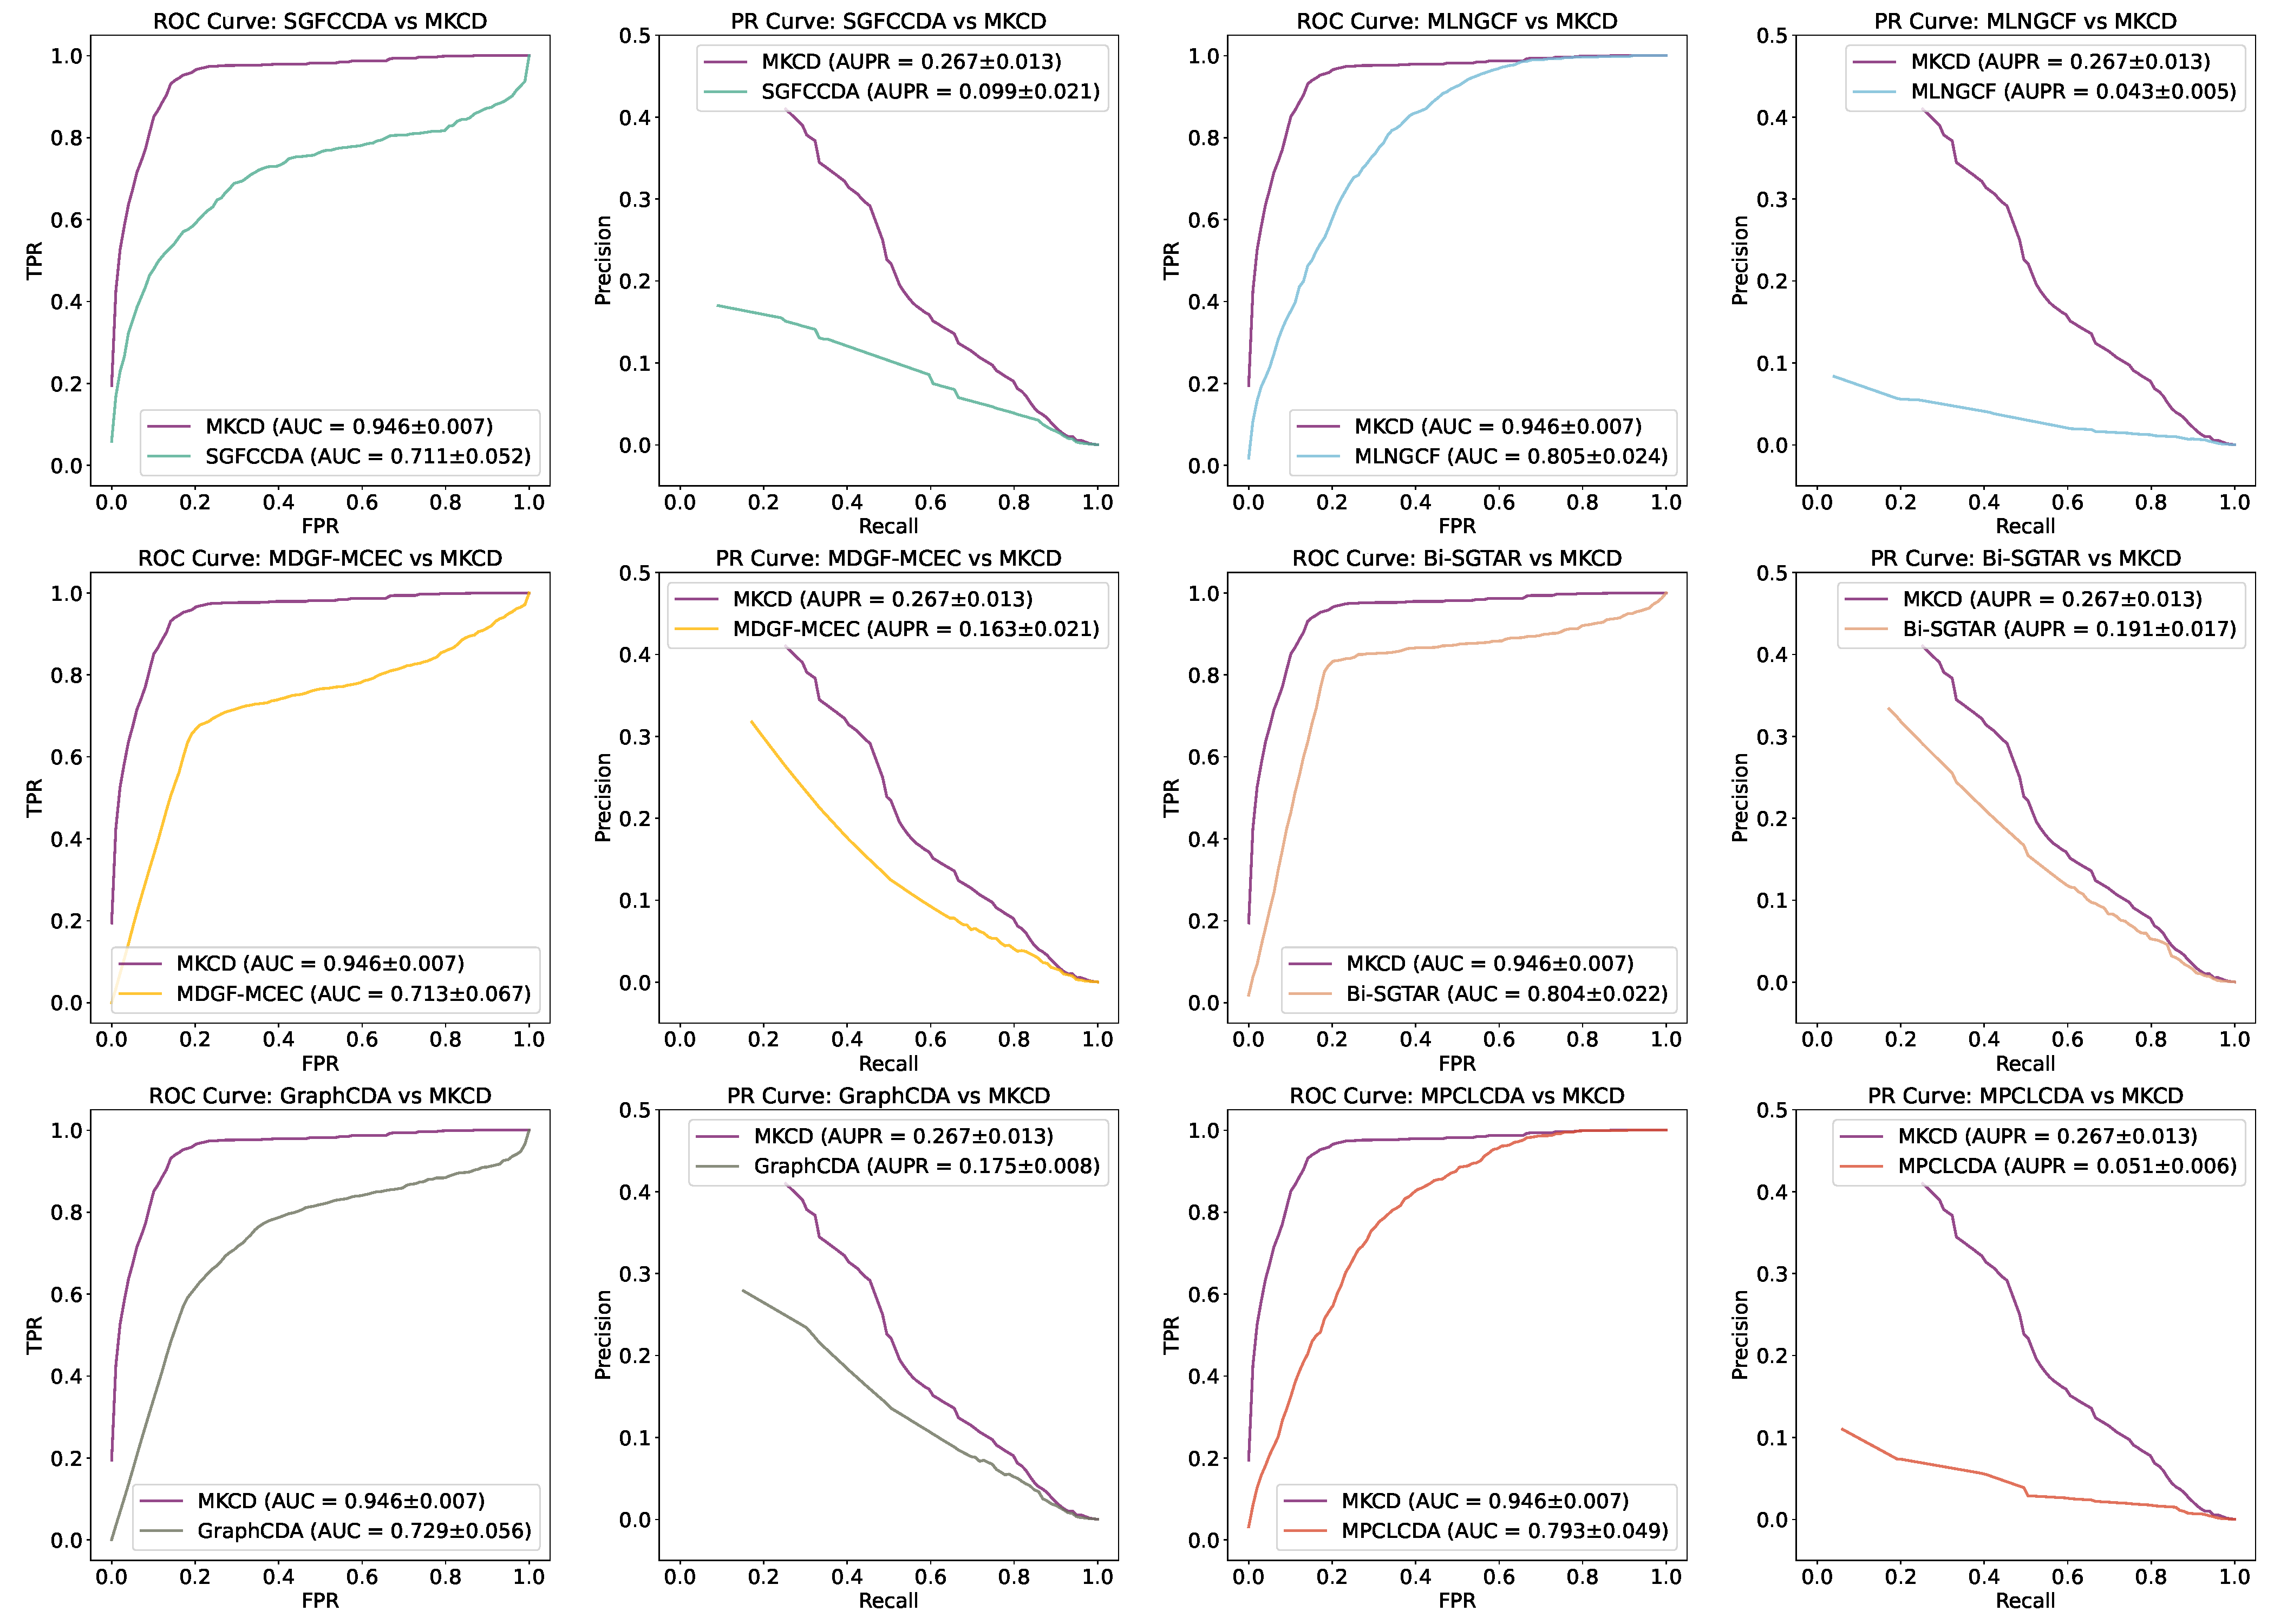
\includegraphics[width=6.2in]{fig/roc_pr_split.pdf}\\
    \caption{ROC and PR curves of MKCD and other comparative methods.}
    \label{fig:roc_pr_split}
\end{figure*}

The learnable parameters for scales 0 to 2 are denoted as $\eta_{0}$, $\eta_{1}$, and $\eta_{2}$, and they are randomly initialized. For each batch of data, we calculate the loss function for circRNA-disease association prediction and update the values of $\eta_{0}\sim\eta_{2}$ using backpropagation. The training process consists of 40 epochs. As shown in Supplementary Figure 3, the values of $\eta_{0}$, $\eta_{1}$, and $\eta_{2}$ fluctuate significantly during the first 10 epochs, gradually converge between epochs 10 and 20, and stabilize after 20 epochs. The final values of $\eta_{0}$, $\eta_{1}$, and $\eta_{2}$ stabilize at 0.295, 0.487, and 0.218, respectively. The experimental results indicate that the weight proportion of the 1-scale neighbor topology embedding is the largest, which is likely because it includes neighbors that are directly connected to the target node, resulting in stronger associations. In contrast, the 2-scale neighbor topology has a smaller weight proportion, possibly due to its indirect, two-step connections to the target node.%*

To evaluate whether RWR (random walk with restart) significantly increases the training and inference time of the model, we compare the model with and without RWR, where the model without RWR is denoted as MKCD\_noRWR. We also replace the KAN network in the pairwise global feature learning module with MLP, denoted as MKCD\_noKAN, to analyze the time cost of KAN. The training time is defined as the time for one epoch, and inference time is the time predict whether a pair of circRNA-disease is associated. As shown in Supplementary Table 7, incorporating RWR adds 0.061 seconds to training time per epoch (an 8.63\% increase) and 0.016 ms to inference time per circRNA-disease pair. The full MKCD model with KAN and RWR increases training time for 40 epochs by approximately 0.105 seconds compared to MKCD\_noKAN (a 15.84\% increase) and requires 0.028 ms more for inference per circRNA-disease pair. These results indicate that RWR and KAN only slightly increased the model's training and inference time.%*

In addition, we also analyze the performance of our model on the larger-scale dataset Pokec \cite{takac2012data}, and the corresponding description is added in Supplementary Table 5.

\subsection{Comparison with other methods}

\begin{table*}[!t]
    \centering
    \renewcommand{\arraystretch}{1.2}
    \begin{threeparttable}[b]
        \caption{Comparison of F1 score and Precision of MKCD with other comparative methods. }\label{tab:tabF1}
        \label{tab:F1}
        \begin{tabular}{p{1.3cm}<{\centering} p{1.9cm}<{\centering}  p{1.9cm}<{\centering} p{1.9cm}<{\centering} p{2.0cm}<{\centering} p{1.9cm}<{\centering} p{1.9cm}<{\centering} p{1.9cm}<{\centering}}
            \hline
            \textbf{} & \textbf{MKCD} & \textbf{SGFCCDA} & \textbf{MLNGCF} & \textbf{MDGF-MCEC} &  \textbf{Bi-SGTAR} & \textbf{GraphCDA} & \textbf{MPCLCDA}\\
            \hline
            F1 & \textbf{0.221} & 0.122 & 0.041 &  0.158 & 0.184 & 0.171 & 0.089\\
            Precision & \textbf{0.162} & 0.092 & 0.042 &  0.116 & 0.141 & 0.148 & 0.069 \\
            \hline
        \end{tabular}
    \end{threeparttable}
    \vspace{-0.4cm}
\end{table*}

\begin{table*}[!t]
    \centering
    \renewcommand{\arraystretch}{1.2}
    \begin{threeparttable}[b]
        \caption{Results of the paired Wilcoxon test comparing MKCD with all other methods. }\label{tab:tab2}
        \label{tab:02}
        \begin{tabular}{p{1.9cm}<{\centering}  p{2.2cm}<{\centering} p{2.2cm}<{\centering} p{2.2cm}<{\centering} p{2.2cm}<{\centering} p{2.2cm}<{\centering} p{2.2cm}<{\centering}}
            \hline
            \textbf{$p$-value} & \textbf{SGFCCDA} & \textbf{MLNGCF} & \textbf{MDGF-MCEC} &  \textbf{Bi-SGTAR} & \textbf{GraphCDA} & \textbf{MPCLCDA}\\
            \hline
            AUC & 2.71e-111 & 7.20e-58 & 2.13e-109 &  3.27e-60 & 6.06e-108 & 1.22e-76 \\
            AUPR & 6.02e-109 & 6.60e-115 & 1.18e-41 &  1.96e-09 & 2.86e-26 & 1.29e-113 \\
            F1 score & 2.20e-56 & 4.38e-98 & 4.72e-30 & 2.57e-08 & 1.52e-04 & 3.43e-79\\
            Precision & 3.66e-83 & 4.22e-114 & 1.80e-47 & 2.47e-20 & 3.24e-33 & 2.52e-103\\
            \hline
        \end{tabular}
    \end{threeparttable}
    \vspace{-0.4cm}
\end{table*}

We compared MKCD with six advanced methods for predicting circRNA-disease associations, including SGFCCD \cite{shang2024sgfccda}, MLNGCF \cite{wu2023mlngcf}, MDGF-MCEC \cite{wu2022mdgf}, Bi-SGTAR \cite{li2024bi}, GraphCDA \cite{dai2022graphcda}, and MPCLCDA \cite{liu2023mpclcda}. Each method was trained using the optimal parameters provided in their original papers, and the same training and testing datasets were utilized in cross-validation to ensure fairness. 

SGFCCDA: This model constructs a circRNA-disease heterogeneous graph and predicts potential circRNA-disease associations through scale graph convolutional networks and convolutional neural networks.

MLNGCF: In this model, various similarities between circRNAs and diseases are utilized to estimate the association scores based on a multilayer attention neural network.

MDGF-MCEC: This method establishes relationship graphs for circRNAs and diseases based on their respective similarities and learns node features through a multi-view dual attention graph convolution network.

Bi-SGTAR: The adjacency matrix of the circRNA-disease heterogeneous graph is decomposed into two views, and an encoder with sparse gating is employed to identify all circRNA-disease associations.

GraphCDA: This approach constructs separate similarity networks for circRNAs and diseases, utilizing a hybrid graph embedding model that combines graph convolutional networks and graph attention networks to simultaneously learn feature representations for circRNAs and diseases.

MPCLCDA: It automatically selects meta-paths for constructing meta-path graphs and employs graph convolutional networks and contrastive learning to learn node features for circRNAs and diseases.

Among them, SGFCCDA, MDGF-MCEC, and GraphCDA are models based on graph convolutional networks, with GraphCDA additionally incorporating an attention mechanism. MPCLCDA is based on contrastive learning methods, while Bi-SGTAR primarily utilizes sparse gating and graph decomposition techniques. %*

\begin{figure*}[!t]
    \centering
    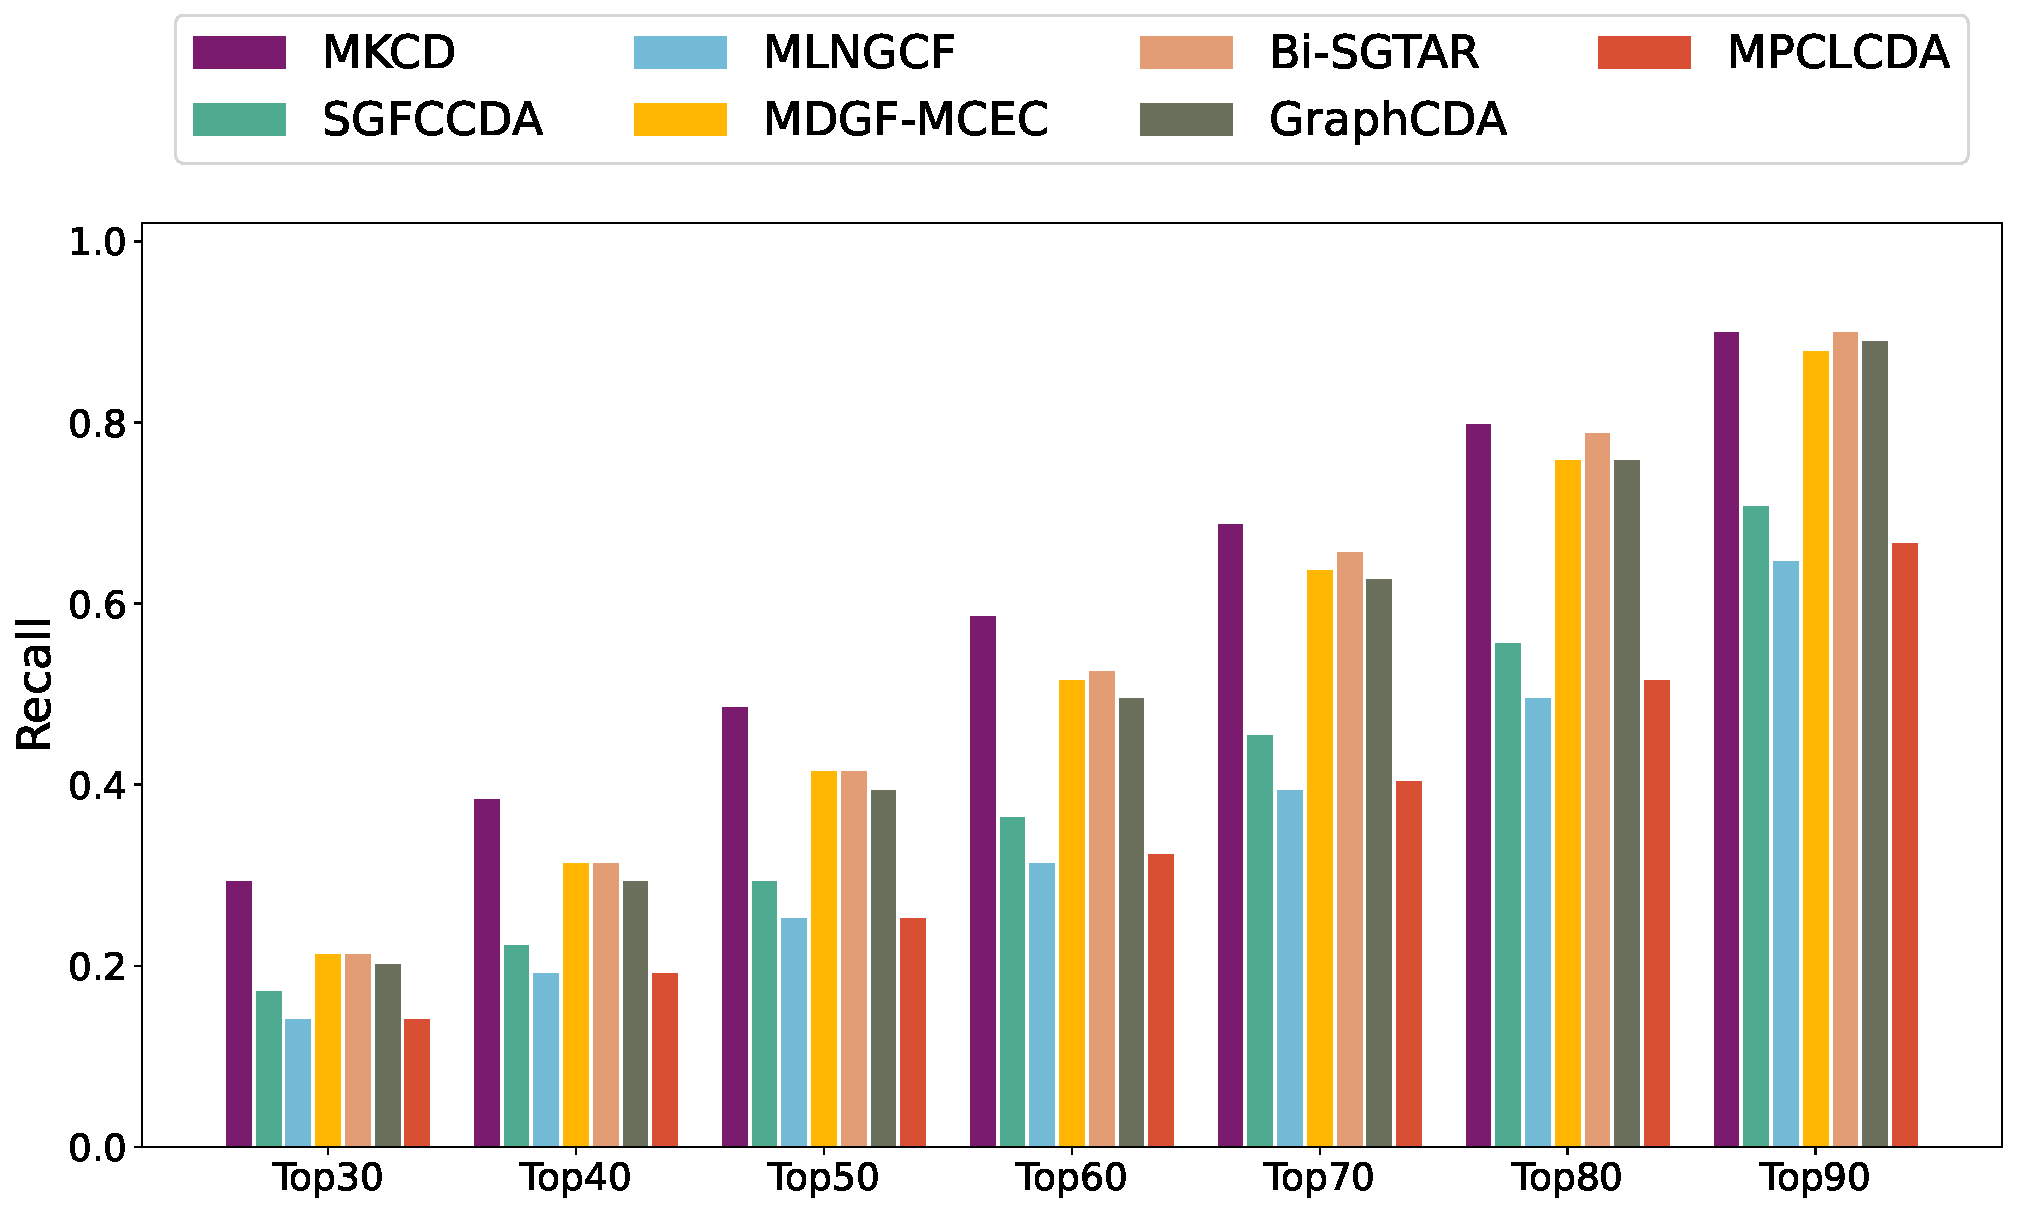
\includegraphics[width=5in]{fig/TopK_Recall.pdf}
     \caption{Recall rates of diseases at multiple top $k$ cutoffs.}
    \label{fig:topK}
	\vspace{-0.4cm}
\end{figure*}

Figure \ref{fig:roc_pr_split} illustrates the ROC and PR curves for MKCD and the other methods. From the figure, it is evident that MKCD achieved the highest average AUC of 0.946, surpassing SGFCCDA by 23.5\%, MLNGCF by 14.1\%, MDGF-MCEC by 23.3\%, Bi-SGTAR by 14.2\%, GraphCDA by 21.7\%, and MPCLCDA by 15.3\%. The average AUPR of MKCD was 0.267, which is higher than SGFCCDA, MLNGCF, MDGF-MCEC, Bi-SGTAR, GraphCDA, and MPCLCDA by 16.8\%, 22.4\%, 10.4\%, 7.6\%, 9.2\%, and 21.6\%, respectively. 
As shown in Table \ref{tab:tabF1}, MKCD also achieves the highest F1 score (F1 = 0.221), which is 9.9\% higher than SGFCCDA, 18.0\% higher than MLNGCF, 6.3\% higher than MDGF-MCEC, 3.7\% higher than Bi-SGTAR, 5.0\% higher than GraphCDA, and 13.2\% higher than MPCLCDA. MKCD achieves the highest Precision of 0.162, outperforming the compared methods by 7.0\%, 12.0\%, 4.6\%, 2.1\%, 1.4\% and 9.3\%, respectively. %*
Both MLNGCF and MPCLCDA employ graph neural networks, focusing solely on integrating the topology and node features of the circRNA-disease heterogeneous graph. In contrast to these two methods, SGFCCDA utilizes scale graph convolutional networks to address the issue of feature mixing between different channels caused by the linear layer structure of graph convolutional networks. MDGF-MCEC and GraphCDA primarily focus on learning from multiple similarity views, while Bi-SGTAR emphasizes learning from multiple heterogeneous graph views, which contributes to their superior performance. Our method outperforms these six methods mainly due to the embedding of multi-scale neighbor topology and the encoding of relationships among multiple features of circRNA, disease, and miRNA nodes.

To evaluate whether the proposed method significantly outperforms the six comparison methods in terms of AUC, AUPR, F1 score, and Precision metrics, we use the paired Wilcoxon test. In 5-fold cross-validation, all seven methods (including the proposed method and six comparison methods) calculate the AUC, AUPR, F1, and Precision scores for 138 diseases. The average score for each method is obtained by averaging the results across five folds, yielding the average score for each method on each disease. Then, for each disease, the score differences between the proposed method and each comparison method on these evaluation metrics are calculated. The absolute values of these differences are ranked, and the signed ranks are used to calculate the test statistic. Finally, the $p$-value is derived using the test statistic and its corresponding distribution to determine whether the proposed method significantly outperforms the comparison methods. According to the results in Table \ref{tab:tab2}, all $p$-values are below 0.05, indicating that MKCD significantly outperforms SGFCCDA, MLNGCF, MDGF-MCEC, Bi-SGTAR, GraphCDA, and MPCLCDA with respect to AUC, AUPR, F1 score, and Precision.%*

For each disease, we calculated the recall rates of circRNA candidates at various top $k$ values (Figure \ref{fig:topK}). When $k = 30$, MKCD achieved a recall rate of 29.3\%, surpassing SGFCCDA by 12.1\%, MLNGCF by 15.2\%, MDGF-MCEC by 8.1\%, Bi-SGTAR by 8.0\%, GraphCDA by 9.1\%, and MPCLCDA by 15.1\%. When $k = 50$, 70, and 90, MKCD maintained its leading position with recall rates of 48.5\%, 68.6\%, and 90.1\%, respectively. Bi-SGTAR (41.3\%, 65.7\%, 89.8\%), MDGF-MCEC (41.3\%, 63.6\%, 87.9\%), and GraphCDA (39.4\%, 62.5\%, 88.8\%) also achieved decent performance. In contrast, SGFCCDA (29.3\%, 45.5\%, 70.6\%), MLNGCF (25.2\%, 39.4\%, 64.6\%), and MPCLCDA (25.3\%, 40.5\%, 66.7\%) showed inferior performance.

\begin{table*}[!t]
    \centering
    \renewcommand{\arraystretch}{1.2}
    \begin{threeparttable}[b]
        \caption{Comparison of AUC, AUPR, F1 score and Precision of MKCD with other comparative methods. }\label{tab:tabCV}
        \label{tab:CV}
        \begin{tabular}{p{1.3cm}<{\centering} p{1.9cm}<{\centering}  p{1.9cm}<{\centering} p{1.9cm}<{\centering} p{2.0cm}<{\centering} p{1.9cm}<{\centering} p{1.9cm}<{\centering} p{1.9cm}<{\centering}}
            \hline
            \textbf{} & \textbf{MKCD} & \textbf{SGFCCDA} & \textbf{MLNGCF} & \textbf{MDGF-MCEC} &  \textbf{Bi-SGTAR} & \textbf{GraphCDA} & \textbf{MPCLCDA}\\
            \hline
            AUC & \textbf{0.956} & 0.852 & 0.789 &  0.728 & 0.813 & 0.713 & 0.801\\
            AUPR &\textbf{0.271} & 0.123 & 0.055 &  0.165 & 0.182 & 0.175 & 0.067\\
            F1 &\textbf{0.269} & 0.130 & 0.076 &  0.143 & 0.187 & 0.179 & 0.086\\
            Precision &\textbf{0.193} & 0.129 & 0.082 &  0.120 & 0.155 & 0.119 & 0.099\\
            \hline
        \end{tabular}
    \end{threeparttable}
    \vspace{-0.4cm}
\end{table*}

To effectively evaluate the model's generalization capability, all known circRNA-disease associations and unknown circRNA-disease association pairs are randomly divided into 60\% training set, 20\% validation set, and 20\% test set. This division ensures that the test set is independent of the training and loss evaluation process. The results (TABLE \ref{tab:tabCV}) indicate that MKCD performs best in terms of AUC, AUPR, F1 score, and Precision, with values of 0.956, 0.271, 0.269, and 0.193, respectively. For AUC, MKCD improves by 10.4\% to 24.3\% compared to other methods, while MKCD's AUPR exceeds other methods by 8.9\% to 21.6\%. MKCD's F1 score outperforms SGFCCDA, MLNGCF, MDGF-MCEC, Bi-SGTAR, GraphCDA, and MPCLCDA by 13.9\%, 19.3\%, 12.6\%, 8.2\%, 9.0\%, and 18.3\%, respectively. MKCD's Precision improves by 6.4\%, 11.1\%, 7.3\%, 3.8\%, 7.4\%, and 9.4\% over other methods. These results demonstrate the excellent generalization ability of MKCD on the independent test set.


To comprehensively evaluate the time efficiency of MKCD and six comparison methods, we analyze their time complexities, where $N$ is the total number of nodes, $d$ is the feature dimension, and the number of circRNA and disease nodes are $n$ and $m$, respectively. As shown in Supplementary Table 11, the time complexity of MKCD is $O(d\cdot N^2)$, while the time complexities of the comparison methods SGFCCDA, MLNGCF, MDGF-MCEC, GraphCDA, and MPCLCDA are all $O(d\cdot N^2)$, and Bi-SGTAR is $O(m\cdot n^2+n\cdot m^2)$. We report the training and inference times of the models, defined as the time to achieve optimal performance and to predict a node pair association, respectively. The training and inference times for MKCD are 30.72 s and 0.352 ms, respectively. Bi-SGTAR, which is primarily based on a sparse gated network, exhibits the highest inference efficiency. GraphCDA, based on a graph convolutional network with shallow network depth, achieves the shortest training time. Overall, the training times for MKCD and the six comparison methods range from 6.67 s to 47.90 s, and the inference times range from 0.068ms to 0.568 ms, all showing high operational efficiency.%*

\begin{table*}[!t]
	\centering
	\renewcommand{\arraystretch}{1.2}
	\begin{threeparttable}[b]
        \caption{Top 15 predicted results of glioma-related circRNAs based on MKCD.}	\label{tab:tab3}
        \label{tab:03}
		\begin{tabular}{p{1cm}<{\centering}  p{2.2cm}<{\centering} p{3.5cm}<{\centering} | p{1cm}<{\centering} p{2.2cm}<{\centering} p{3.5cm}<{\centering}}
            \hline
            Rank & CircRNA name & Evidence & Rank &	CircRNA name & Evidence \\
            \hline
            1 & circ\_002136 & \ $L^a$, PMID:30736838 & 9 & hsa\_circ\_0079593 & \ $L^a$, PMID:31148222 \\
            2 & hsa\_circ\_0061868 & \ PMID:30341906 & 10 & circSMO742 & \ $L^a$, PMID:31895689 \\
            3 & circPTN & \ $L^a$, PMID:31511040 & 11 & hsa\_circ\_0012129 & \ $L^a$, PMID:29686222 \\
            4 & circ-TTBK2 & \ $L^a$, PMID:32196629 & 12 & hsa\_circ\_0088732 & \ $L^a$, PMID:32154171 \\
            5 & circ-EZH2 & \ $L^a$, PMID:31669648 & 13 & circNFIX & \ $L^a$, PMID:30072869 \\
            6 & hsa\_circ\_0000594 & \ $L^a$, PMID:28219405 & 14 & circ-PTPRZ1 & \ $L^a$, PMID:31364003 \\
            7 & hsa\_circ\_0005198 & \ $L^a$, PMID:31038801 & 15 & hsa\_circ\_0014359 & \ $L^a$, PMID:30745107 \\
            8 & hsa\_circ\_0000177 & \ $L^a$, PMID:30010402 & & & \\
             \hline
		\end{tabular}
	\end{threeparttable}
    \begin{flushleft}
        \ \ \ \ \ \ \ \ \ \ \ $L^a$: circRNADisease v2.0.
    \end{flushleft}
    \vspace{-0.4cm}
\end{table*}

\begin{table*}[!t]
	\centering
	\renewcommand{\arraystretch}{1.2}
	\begin{threeparttable}[b]
        \caption{Top 15 predicted results of systemic lupus erythematosus-related circRNAs based on MKCD.}	
        \label{tab:04}
		\begin{tabular}{p{1cm}<{\centering}  p{2.2cm}<{\centering} p{3.5cm}<{\centering} | p{1cm}<{\centering} p{2.2cm}<{\centering} p{3.5cm}<{\centering}}
            \hline
            Rank & CircRNA name & Evidence & Rank &	CircRNA name & Evidence \\
            \hline
            1 & hsa\_circ\_0046599 & \ $L^a$, PMID:29360436 & 9 & hsa\_circ\_0008615 & \ $L^a$, PMID:29360436 \\
            2 & hsa\_circ\_0001866 & \ $L^a$, PMID:29360436 & 10 & hsa\_circ\_0021549 & \ $L^a$, PMID:29360436 \\
            3 & hsa\_circ\_0034398 & \ $L^a$, PMID:29360436 & 11 & has\_circ\_0049220 & \ $L^a$, PMID:29606700 \\
            4 & hsa\_circ\_0003146 & \ $L^a$, PMID:29360436 & 12 & hsa\_circ\_0092374 & \ $L^a$, PMID:29360436 \\
            5 & hsa\_circ\_0000479 & \ $L^a$, PMID:31608065 & 13 & hsa\_circ\_0040705 & \ $L^a$, PMID:29360436 \\
            6 & hsa\_circ\_0057762 & \ $L^a$, PMID:30628013 & 14 & hsa\_circ\_0012919 & \ $L^a$, PMID:30237316 \\
            7 & circPTPN22 & \ $L^a$, PMID:30871426 & 15 & hsa\_circ\_0049224 & \ $L^a$, PMID:29606700 \\
            8 & hsa\_circ\_0045272 & \ $L^a$, PMID:29700819 & & & \\
            \hline
		\end{tabular}
	\end{threeparttable}
    \begin{flushleft}
        \ \ \ \ \ \ \ \ \ \ \ $L^a$: circRNADisease v2.0.
    \end{flushleft}
    \vspace{-0.4cm}
\end{table*}

\begin{table*}[!t]
	\centering
	\renewcommand{\arraystretch}{1.2}
	\begin{threeparttable}[b]
        \caption{Top 15 predicted results of glioblastoma-related circRNAs based on MKCD.}	\label{tab:tab4}
        \label{tab:05}
		\begin{tabular}{p{1cm}<{\centering}  p{2.2cm}<{\centering} p{3.5cm}<{\centering} | p{1cm}<{\centering} p{2.2cm}<{\centering} p{3.5cm}<{\centering}}
            \hline
            Rank & CircRNA name & Evidence & Rank &	CircRNA name & Evidence \\
            \hline
            1 & hsa\_circ\_0001801 & \ $L^a$, PMID:31858556 & 9 & circMTO1 & \ $L^a$, PMID:31456594 \\
            2 & circNT5E & \ $L^a$, PMID:29967262 & 10 & circ-AKT3 & \ $L^a$, PMID:31470874 \\
            3 & circ-PITX1 & \ $L^a$, PMID:31493405 & 11 & circPVT1 & \ unconfirmed \\
            4 & hsa\_circ\_0043949 & \ $L^a$, PMID:31823158 & 12 & circPTN & \ $L^a$, PMID:31511040 \\
            5 & hsa\_circ\_0074027 & \ $L^a$, PMID:30738578 & 13 & hsa\_circ\_101996 & \ unconfirmed \\
            6 & circMMP9 & \ $L^a$, PMID:30470262 & 14 & hsa\_circ\_100242 & \ unconfirmed \\
            7 & circ-Foxo3 & \ $L^a$, PMID:31802888 & 15 & hsa\_circ\_0003855 & \ unconfirmed \\
            8 & hsa\_circ\_0001946 & \ $L^a$, PMID:31599076 & & & \\
             \hline
		\end{tabular}
	\end{threeparttable}
    \begin{flushleft}
        \ \ \ \ \ \ \ \ \ \ \ $L^a$: circRNADisease v2.0.
    \end{flushleft}
    \vspace{-0.4cm}
\end{table*}

\subsection{Case studies on three diseases}

We conducted case studies on glioma, systemic lupus erythematosus, and glioblastoma to further validate MKCD’s ability to mine potential circRNA candidates associated with these diseases. Glioma and glioblastoma are two types of primary brain tumors \cite{weller2015glioma, wirsching2017glioblastoma}, while systemic lupus erythematosus is a systemic autoimmune disease, primarily affecting women \cite{kaul2016systemic}. For each disease, the circRNA candidates were ranked in descending order based on their association scores, and the top 15 circRNAs were selected as candidates. Tables \ref{tab:03}, \ref{tab:04}, and \ref{tab:05} show the top 15 circRNA candidates for glioma, systemic lupus erythematosus, and glioblastoma, respectively. The circRNADisease v2.0 database provides validated associations between circRNAs and various diseases, covering 4246 circRNAs and 330 diseases \cite{fan2022circr2disease}. This database, along with relevant bioinformatics literature, was used to validate the predictions of circRNA-disease associations.

Using glioma as an example (Table \ref{tab:03}), all 15 circRNAs are validated in the literature, with 14 of them have been identified in circRNADisease v2.0. For instance, the top-ranked circ\_002136 was found by He {\it et al.} \cite{he2019fus} to inhibit the viability, migration, and tube formation of U87 glioma-exposed endothelial cells (GECs). Li {\it et al.} \cite{li2019circ} found that the expression levels of hsa\_circ\_0061868 were upregulated in glioma cells.

All 15 circRNA candidates associated with systemic lupus erythematosus (SLE) (Table \ref{tab:04}) are confirmed in the literature and have been included in circRNADisease v2.0. For example, Li {\it et al.} \cite{li2018comprehensive} identified hsa\_circ\_0046599 as a potential biomarker for systemic lupus erythematosus. Hsa\_circ\_0000479 was confirmed by Guo {\it et al.} \cite{guo2019hsa_circ_0000479} to be upregulated in peripheral blood mononuclear cells of patients with SLE.

For glioblastoma, 11 of the top 15 circRNA candidates (Table \ref{tab:05}) are validated in recent literature and documented in circRNADisease v2.0. For example, the study by Wang {\it et al.} \cite{wang2018circnt5e} demonstrated that circNT5E exhibits tumor suppressor-like features in glioblastoma. Additionally, circMMP9 has been shown by Wang {\it et al.} \cite{wang2018eif4a3} to promote the proliferation, migration, and invasion of glioblastoma multiforme cells. 
The unverified hsa\_circ\_101996 shares the same gene symbol as circSPECC1, which is shown to inhibit the proliferation, migration, invasion, and colony formation abilities of glioblastoma cells by encoding a new protein named SPECC1-415aa \cite{wei2024novel}. This suggests that hsa\_circ\_101996 is likely associated with glioblastoma. The unverified circPVT1, hsa\_circ\_100242, and hsa\_circ\_0003855 were ranked in the top 15 by Bi-SGTAR, and in the top 20 by MDGF-MCEC and GraphCDA, while SGFCCDA, MLNGCF, and MPCLCDA rank them among the top 30 disease-related circRNA candidates. This rankings indicates that both our method and the six comparative methods consider these unverified circRNA candidates as highly likely candidates for glioblastoma association.
 

\subsection{Prediction of novel circRNA-disease associations}
We utilized all known associations between circRNAs and diseases, and randomly selected an equal number of negative examples to train MKCD to predict circRNA candidates for 138 diseases. The top 15 circRNA candidates predicted by MKCD for each disease are listed in Supplementary File SF1.

\section{Conclusions}
This paper presents a novel approach for encoding the relationships among circRNA, miRNA, and disease node features, while effectively learning and integrating both global and local features of node pairs to predict disease-related circRNAs. By adjusting the walking range of random walkers in the circRNA-disease-miRNA heterogeneous graph, multi-scale neighbor topologies are constructed, and the importance of each scale-specific neighbor topology is adaptively determined. The proposed multi-scale neighbor topology-guided transformer dynamically updates the neighbor topology and captures the evolving relationships between the features of circRNA, miRNA, and disease nodes. The FGN assigns higher weights to topological and original features based on their importance. The ACK encodes the features of circRNA-disease node pairs, facilitating the identification of local and global dependencies among pairwise attributes. The comparison results show that our model outperforms other state-of-the-art methods in terms of AUC and AUPR. The recall rate of top-ranked circRNA candidates and case studies over three diseases further prove that MKCD is capable of providing reliable diseaserelated circRNA candidates. 
With the increasing availability of circRNA-diseases association data, our future work will focus on developing advanced methods for accurate prediction of circRNA-disease associations in large-scale datasets.
\bibliographystyle{IEEEtran}
\bibliography{cas-refs}
\end{document}
